\chapter{Experiments}
\label{ch:experiments}
\section{Qualisys optical motion tracker}
\indent The Qualisys optical motion tracking system uses high speed digital cameras to capture the motion of a measurement object with passive or active markers attached.
The technology is precise and robust and delivers high quality data to the observer in real-time. The provided software tools allows to perform basic motion calculations, such as speed, acceleration, rotation and angle, as well as other more complex calculations. The system has eight cameras which are distributed around a room. The precision of this system allows its use as a reference system to evaluate portable motion tracking systems such as the GaitWatch.

\begin{figure}[H]
\centering
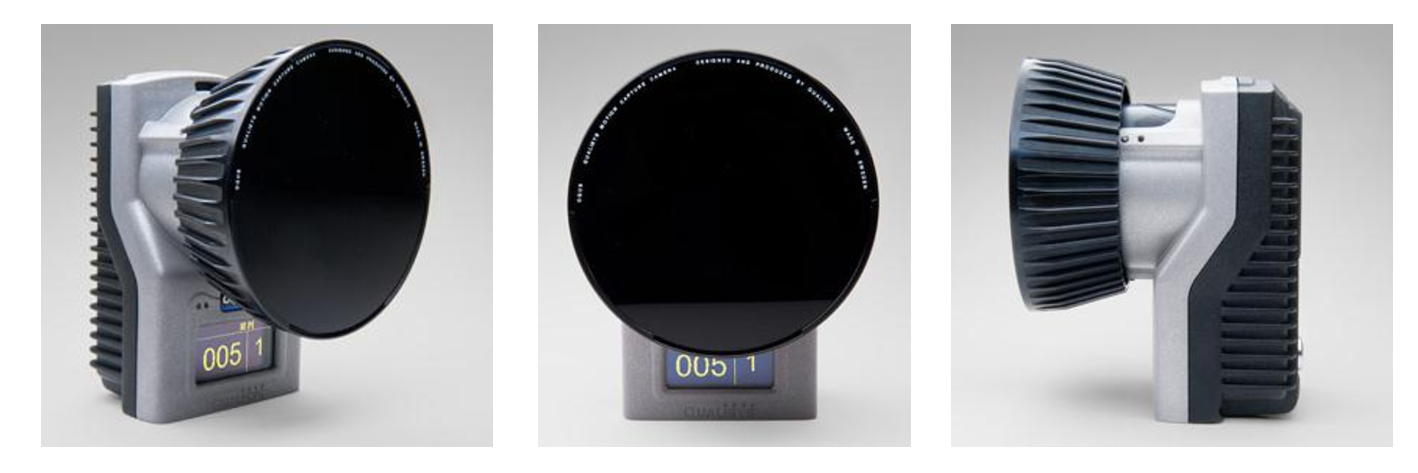
\includegraphics[width=0.7\textwidth]{figures/qs_cameras}
\caption{An Oqus camera part of the Qualisys system.}
\label{fig:qs_cameras}
\end{figure}

\subsection{Computing Euler angles using Qualisys data}
\indent \indent If the subject is wearing two markers per segment, then the pitch angle of such segment is computed between the vector defined by the upper and lower markers and the vector normal to the Earth's surface. To be able to compute it we first have to define a third point which has the same X coordinate as the lower marker and the same Z coordinate as the upper marker. This will define a right triangle in which one of the contiguous cathetus is normal to the Earth's surface and the hypotenuse is defined by the line between the upper and the lower point. Therefore, by calculating the arctangent we can easily find the angle of the right triangle, which is, in turn, the pitch angle. Figure \ref{fig:pitch_triangle} shows this process.

\begin{figure}[H]
\centering
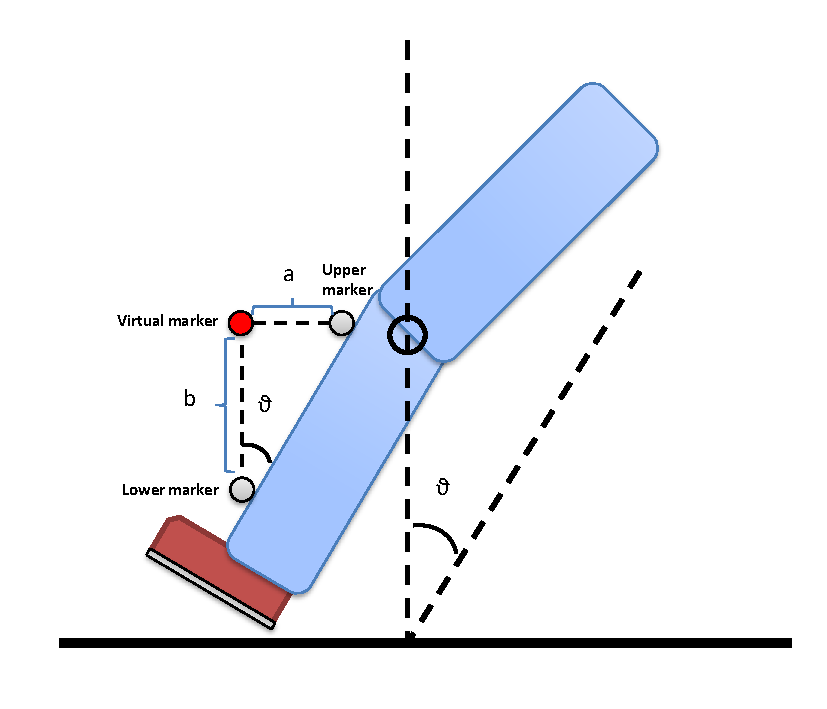
\includegraphics[width=0.7\textwidth]{figures/qualisys_pitch}
\caption{Diagram of the pitch computation using the Qualisys system.}
\label{fig:pitch_triangle}
\end{figure}

\indent Therefore, the pitch angle is computed applying,

\begin{gather}
\theta = \arctan\left(\frac{a}{b}\right)\\
a=\sqrt{\left(x_{upper}-x_{lower}\right)^2+\left(z_{upper}-z_{upper}\right)^2}\\
b=\sqrt{\left(x_{lower}-x_{lower}\right)^2+\left(z_{lower}-z_{upper}\right)^2}
\label{eq:qs_pitch}
\end{gather}

where $[x_{lower},z_{lower}]$ and $[x_{upper},z_{upper}]$ are the coordinates of the projections of the lower and upper markers in the XZ plane, respectively.

\section{Qualisys validation experiments}
\subsection{Data gathering protocol}
\begin{itemize}
\item Switch on the computer.
\item Switch on the Qualisys system.
\item Start the computer and select the "Tracking" account.
\item Write any password, the system will say that the password is wrong and it will show the secret question. The answer to the secret question is "tracking".
\item Once the session has started, open the "Qualisys Track Manager". 
\item Place the calibration frame (which is in the big metallic box and has an L shape) on the floor. 
\item Press the red button and check that the maximum number of cameras see the four markers which are attached to the calibration frame. You may need to adjust the position of the cameras. The cameras also have a small display which show the ID of the camera and the number of markers which are seen in each instant.
\item When all the cameras are ready, go to "capture$\rightarrow$calibrate". Select the desired delay and the desired calibration time (30 seconds should be fine). 
\item Grab the calibration wand (the device which is shaped as a T), click the button to start the calibration and move around the room moving the wand trying to cover all the space.
\item When the calibration is done, hide both the calibration frame and the calibration wand somewhere where the markers are not seen by the cameras (you may need to put them back into the big metallic box or just put them out of the room).
\item The system is now ready to start the measurements.
\item Place the GaitWatch system on the subject and place the markers on the desired segments of the subject. 
\item Press the red button (new capture) and complete the required fields: initial delay, number of samples (200 by default), duration and name of the file. 
\item Before starting the capture, switch on the GaitWatch system and press the button to start the measurement. Tell the subject to stay static.
\item Go back to the computer, start the capture and write down the current time together with the name you have given to the file. 
\item The subject may now move around the room and carry out the movements he is instructed to. 
\item When the capture is done, press the GaitWatch button again to stop the measurement. 
\item Go back to the computer and label one by one all the markers that were identified by the program. This is done by clicking on the markers, going to "identify$\rightarrow$label. 
\item Once all the markers are identified, save the file and go to "file$\rightarrow$export$\rightarrow$MAT", then click OK. This will export all the data to a .mat file. Be careful because the .mat file is created when we start a new capture but it will remain empty until the exportation. 
\end{itemize}

The next step would be to download the GaitWatch data to the computer. To do so we use the \textit{GW\_comm.m} routine. This routine will also ask the user to give each one of the files a number. Be sure to give the file the same number which was given to the Qualisys file. Once all the data are identified, we can run the \textit{param\_optimization.m} routine which loads both the GaitWatch and Qualisys data, synchronizes them and computes the optimal parameters of the algorithm used to compute the orientation using the GaitWatch data. \\

\indent The following sections contain a set of figures depicting the pitch angle of different segments computed using both the Qualisys and the GaitWatch systems. 

\section{Fast Walking}

\begin{figure}[H]
\centering
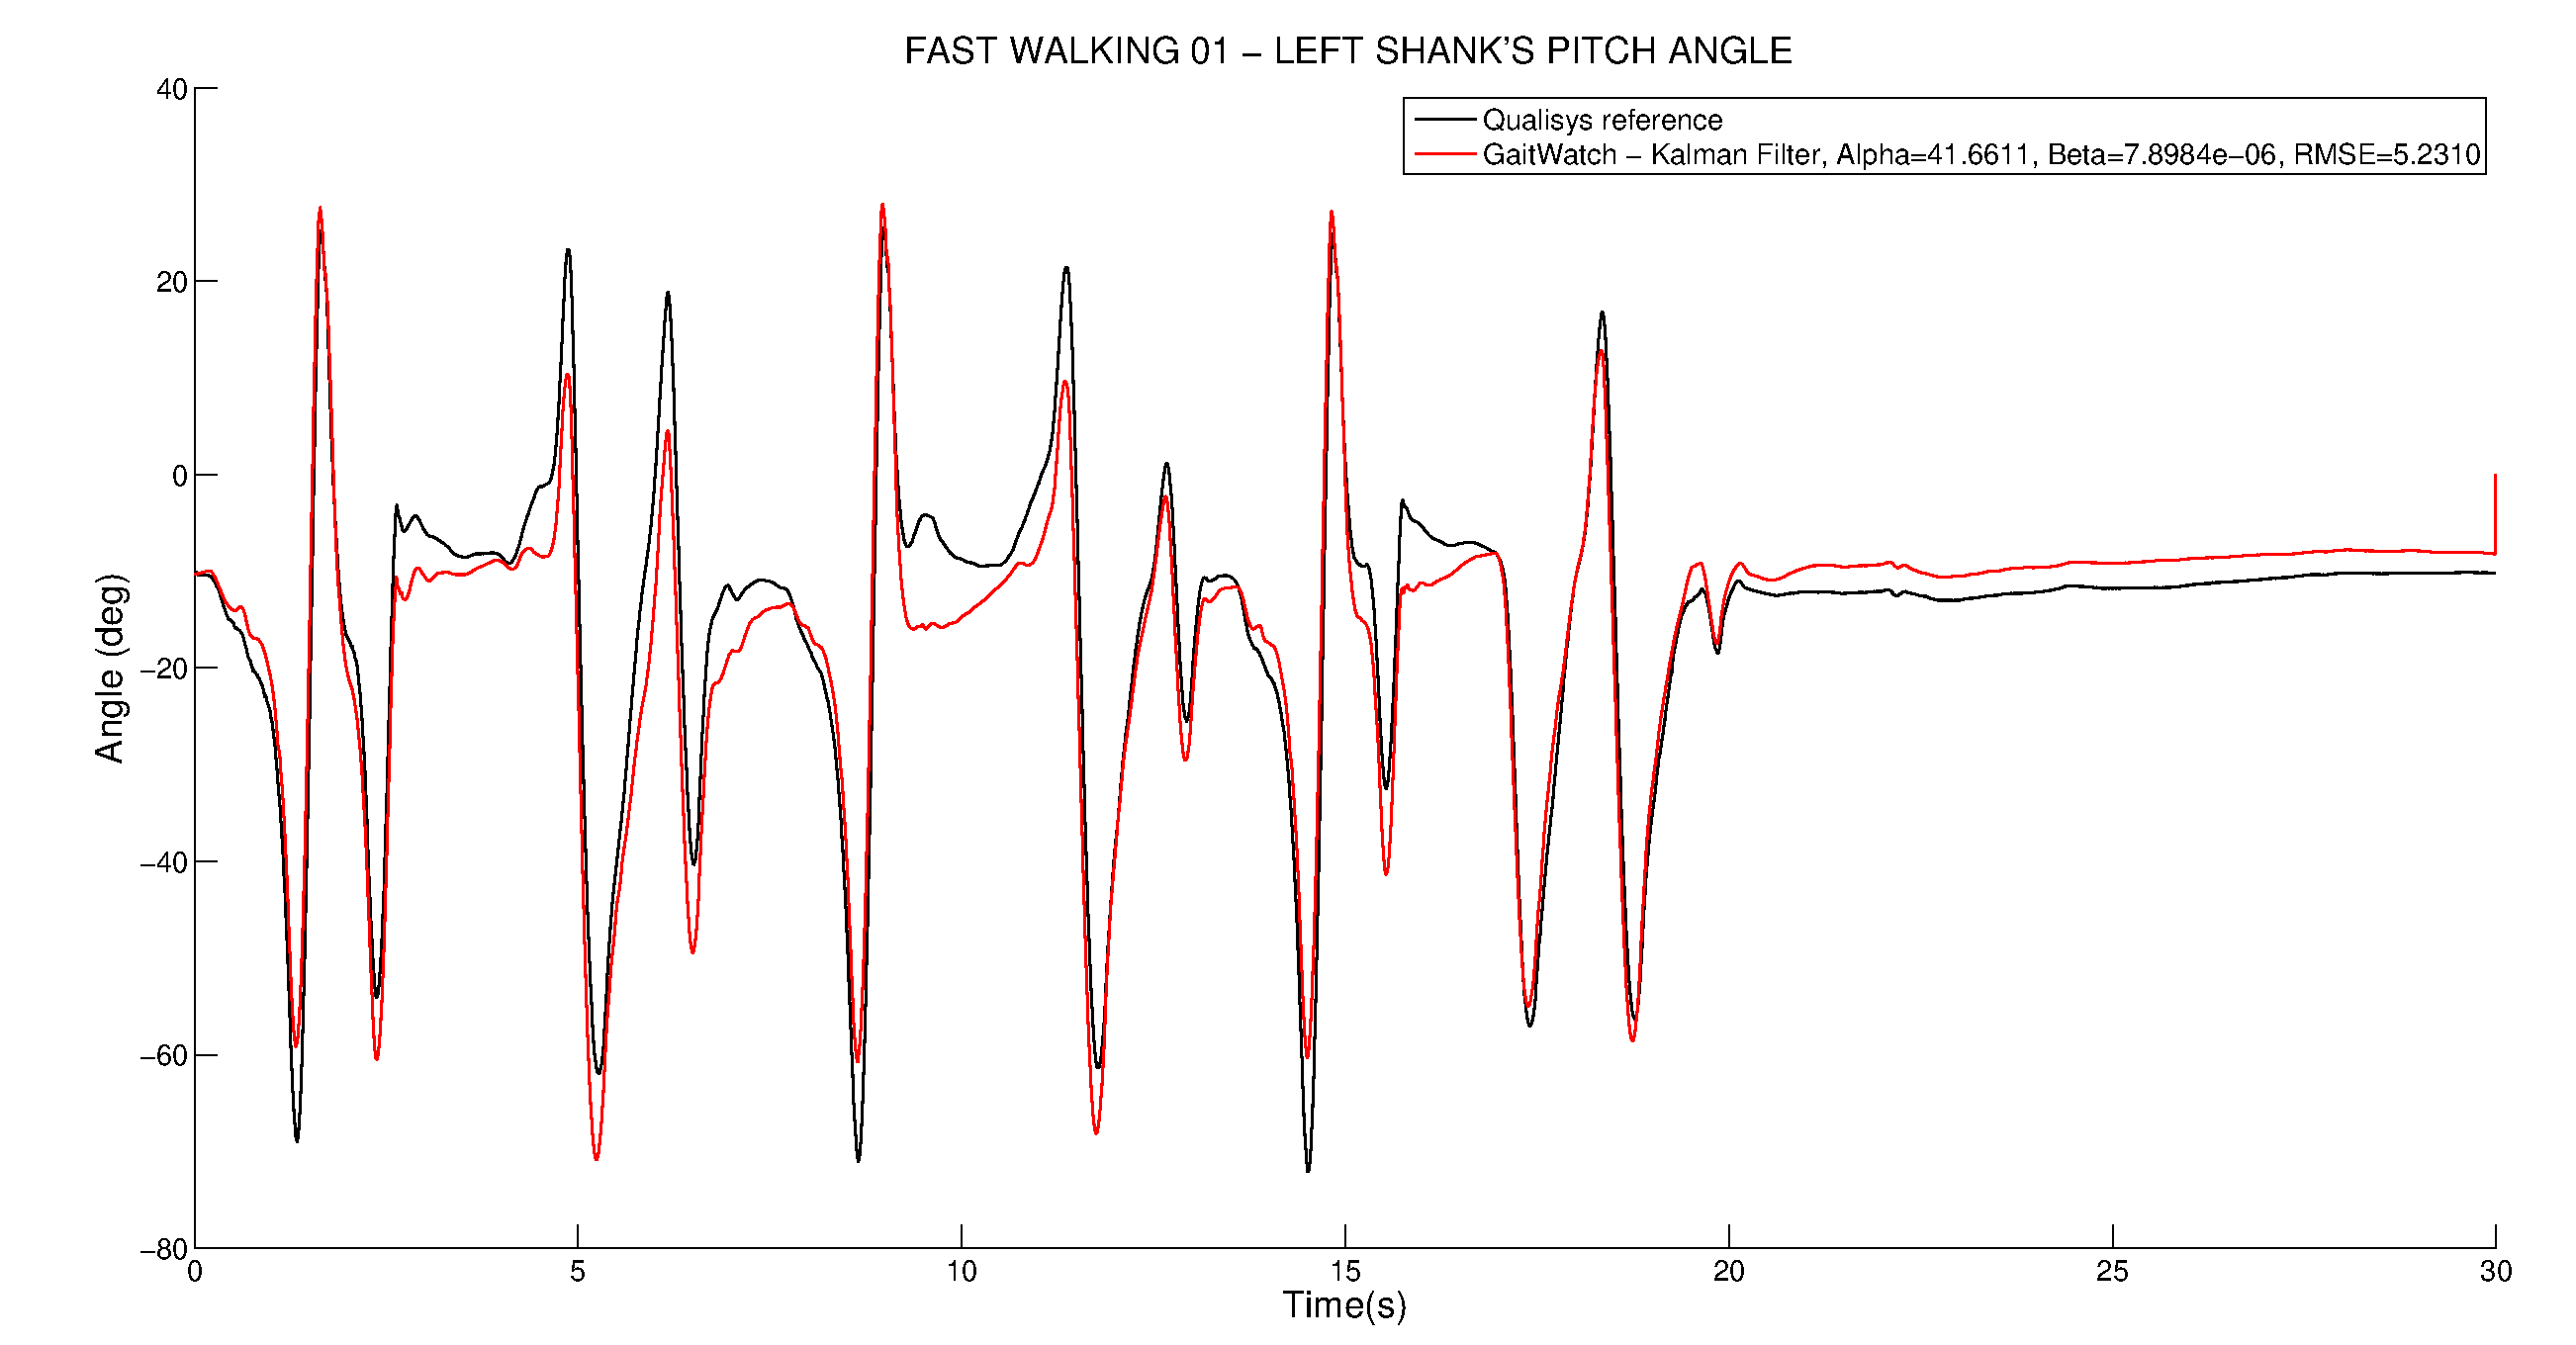
\includegraphics[width=1\textwidth]{figures/fast_walking_01_left_shank.eps}
\caption{Pitch angle of left shank measured while walking fast (GaitWatch vs. Qualisys).}
\label{fig:fast_walking_left_shank01}
\end{figure}

\begin{figure}[H]
\centering
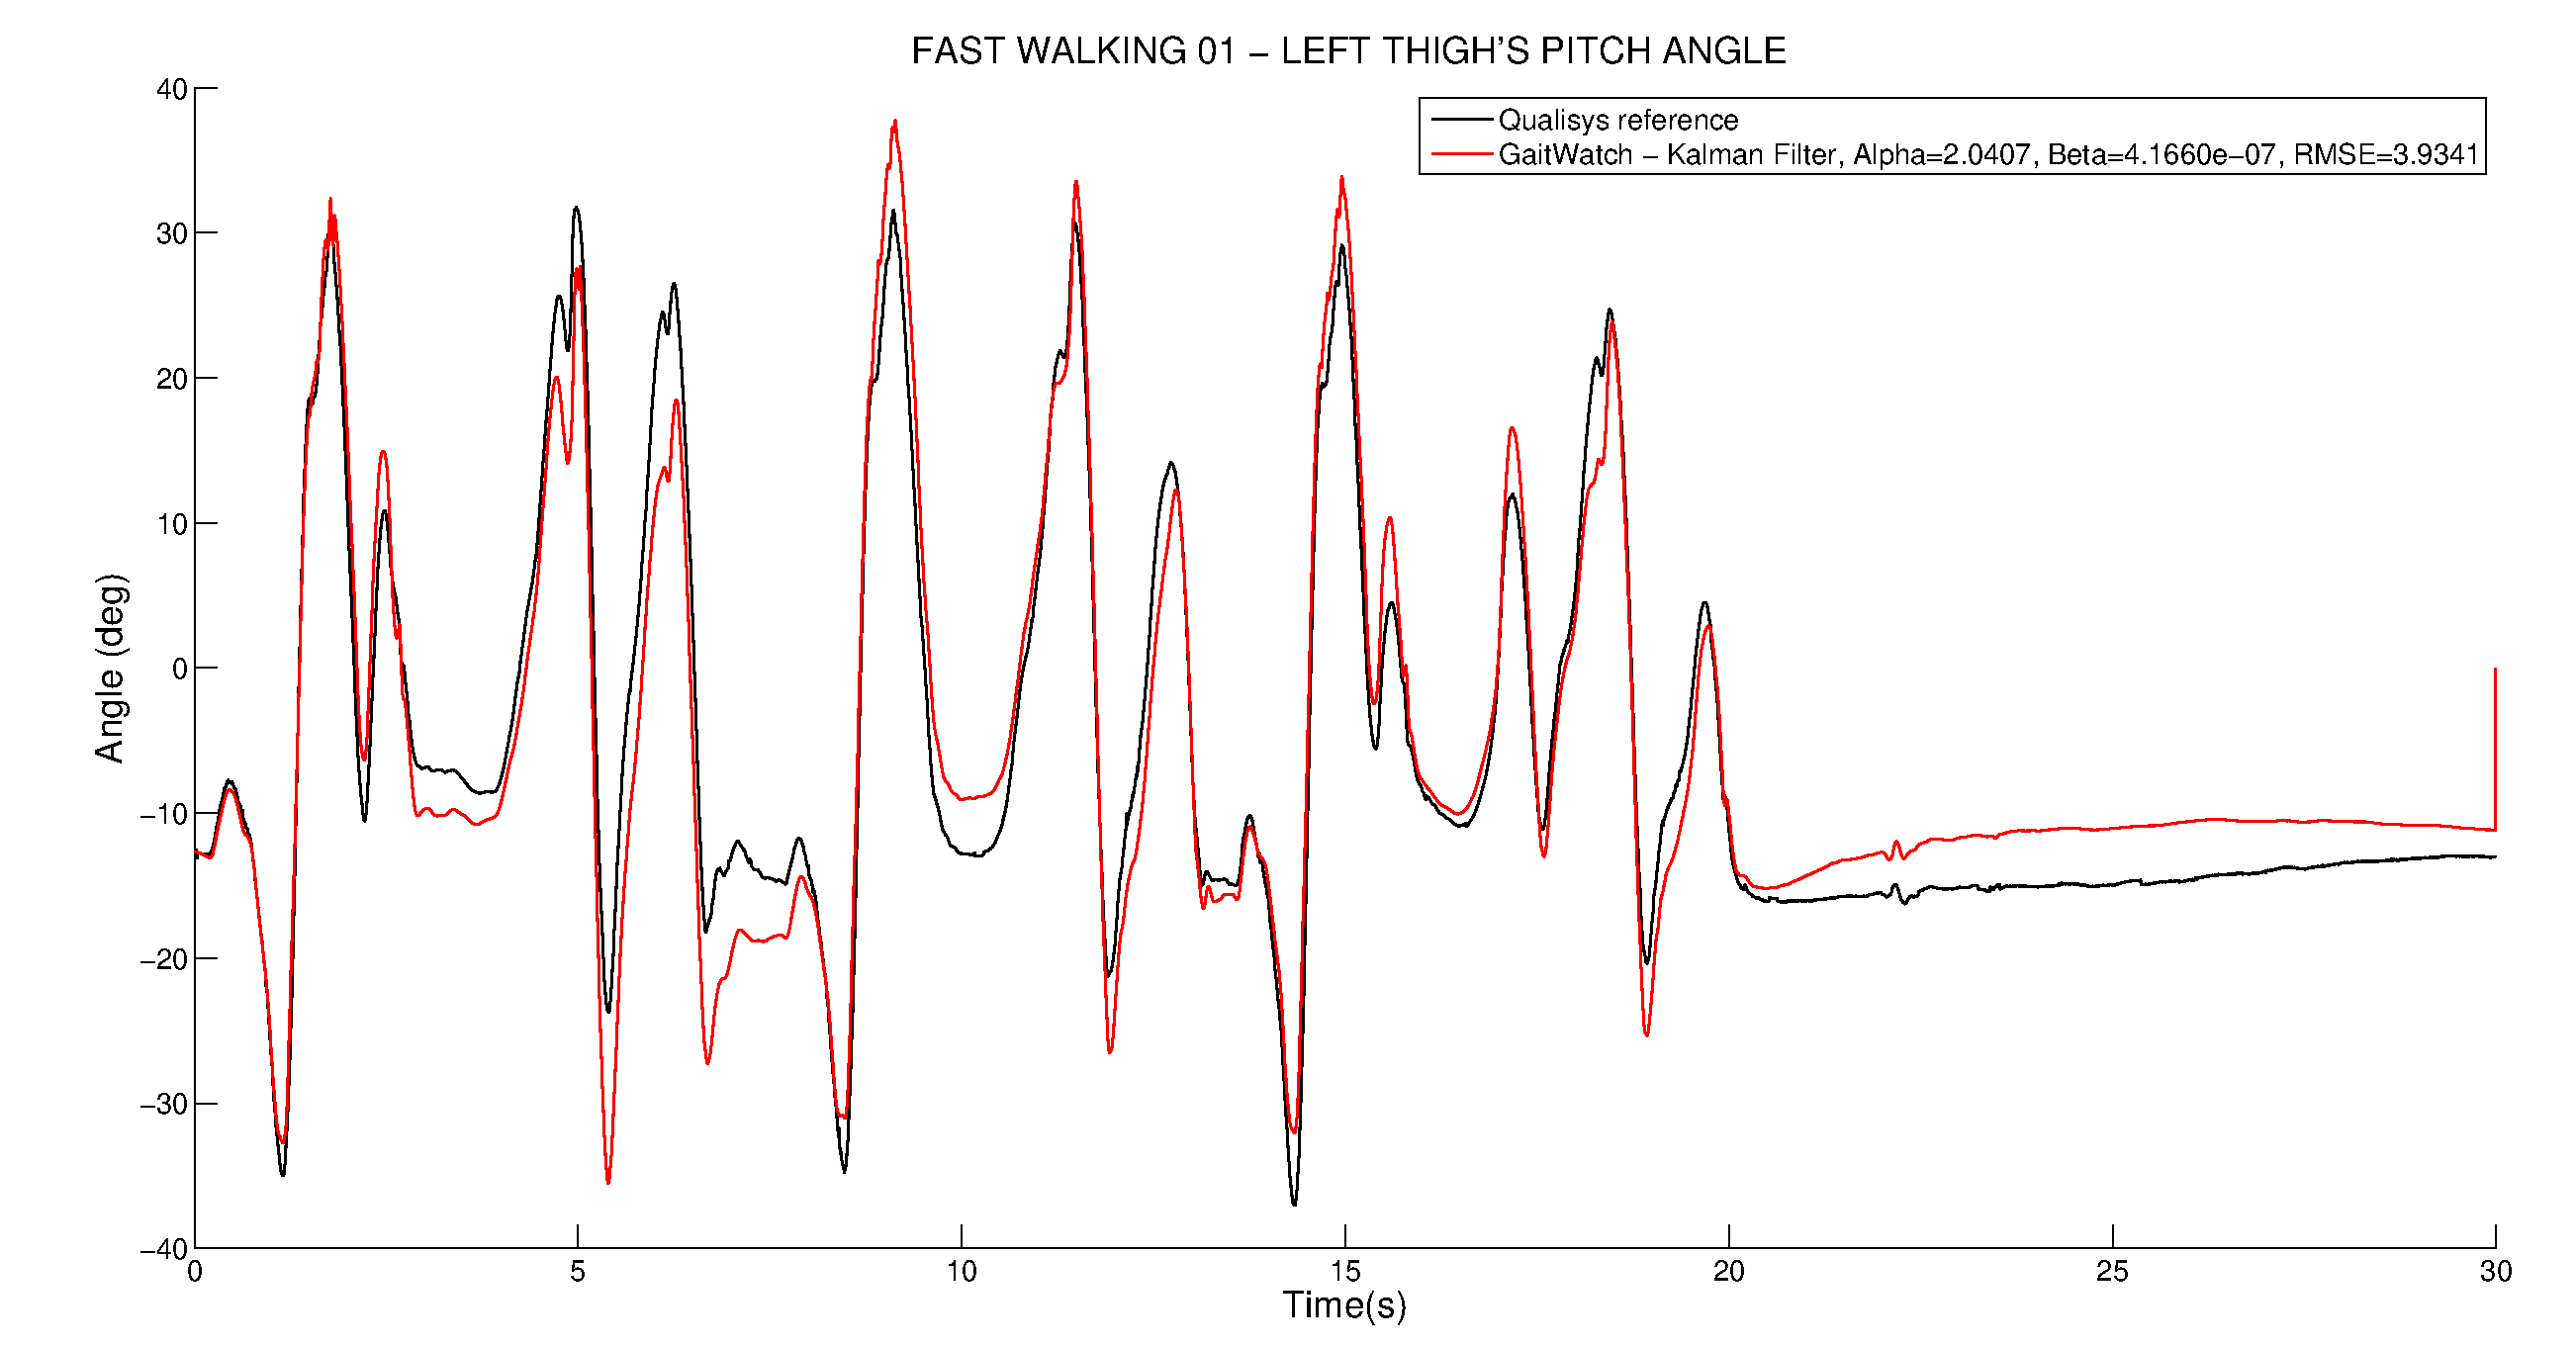
\includegraphics[width=1\textwidth]{figures/fast_walking_01_left_thigh.eps}
\caption{Pitch angle of left thigh measured while walking fast (GaitWatch vs. Qualisys).}
\label{fig:fast_walking_left_thigh01}
\end{figure}

\begin{figure}[H]
\centering
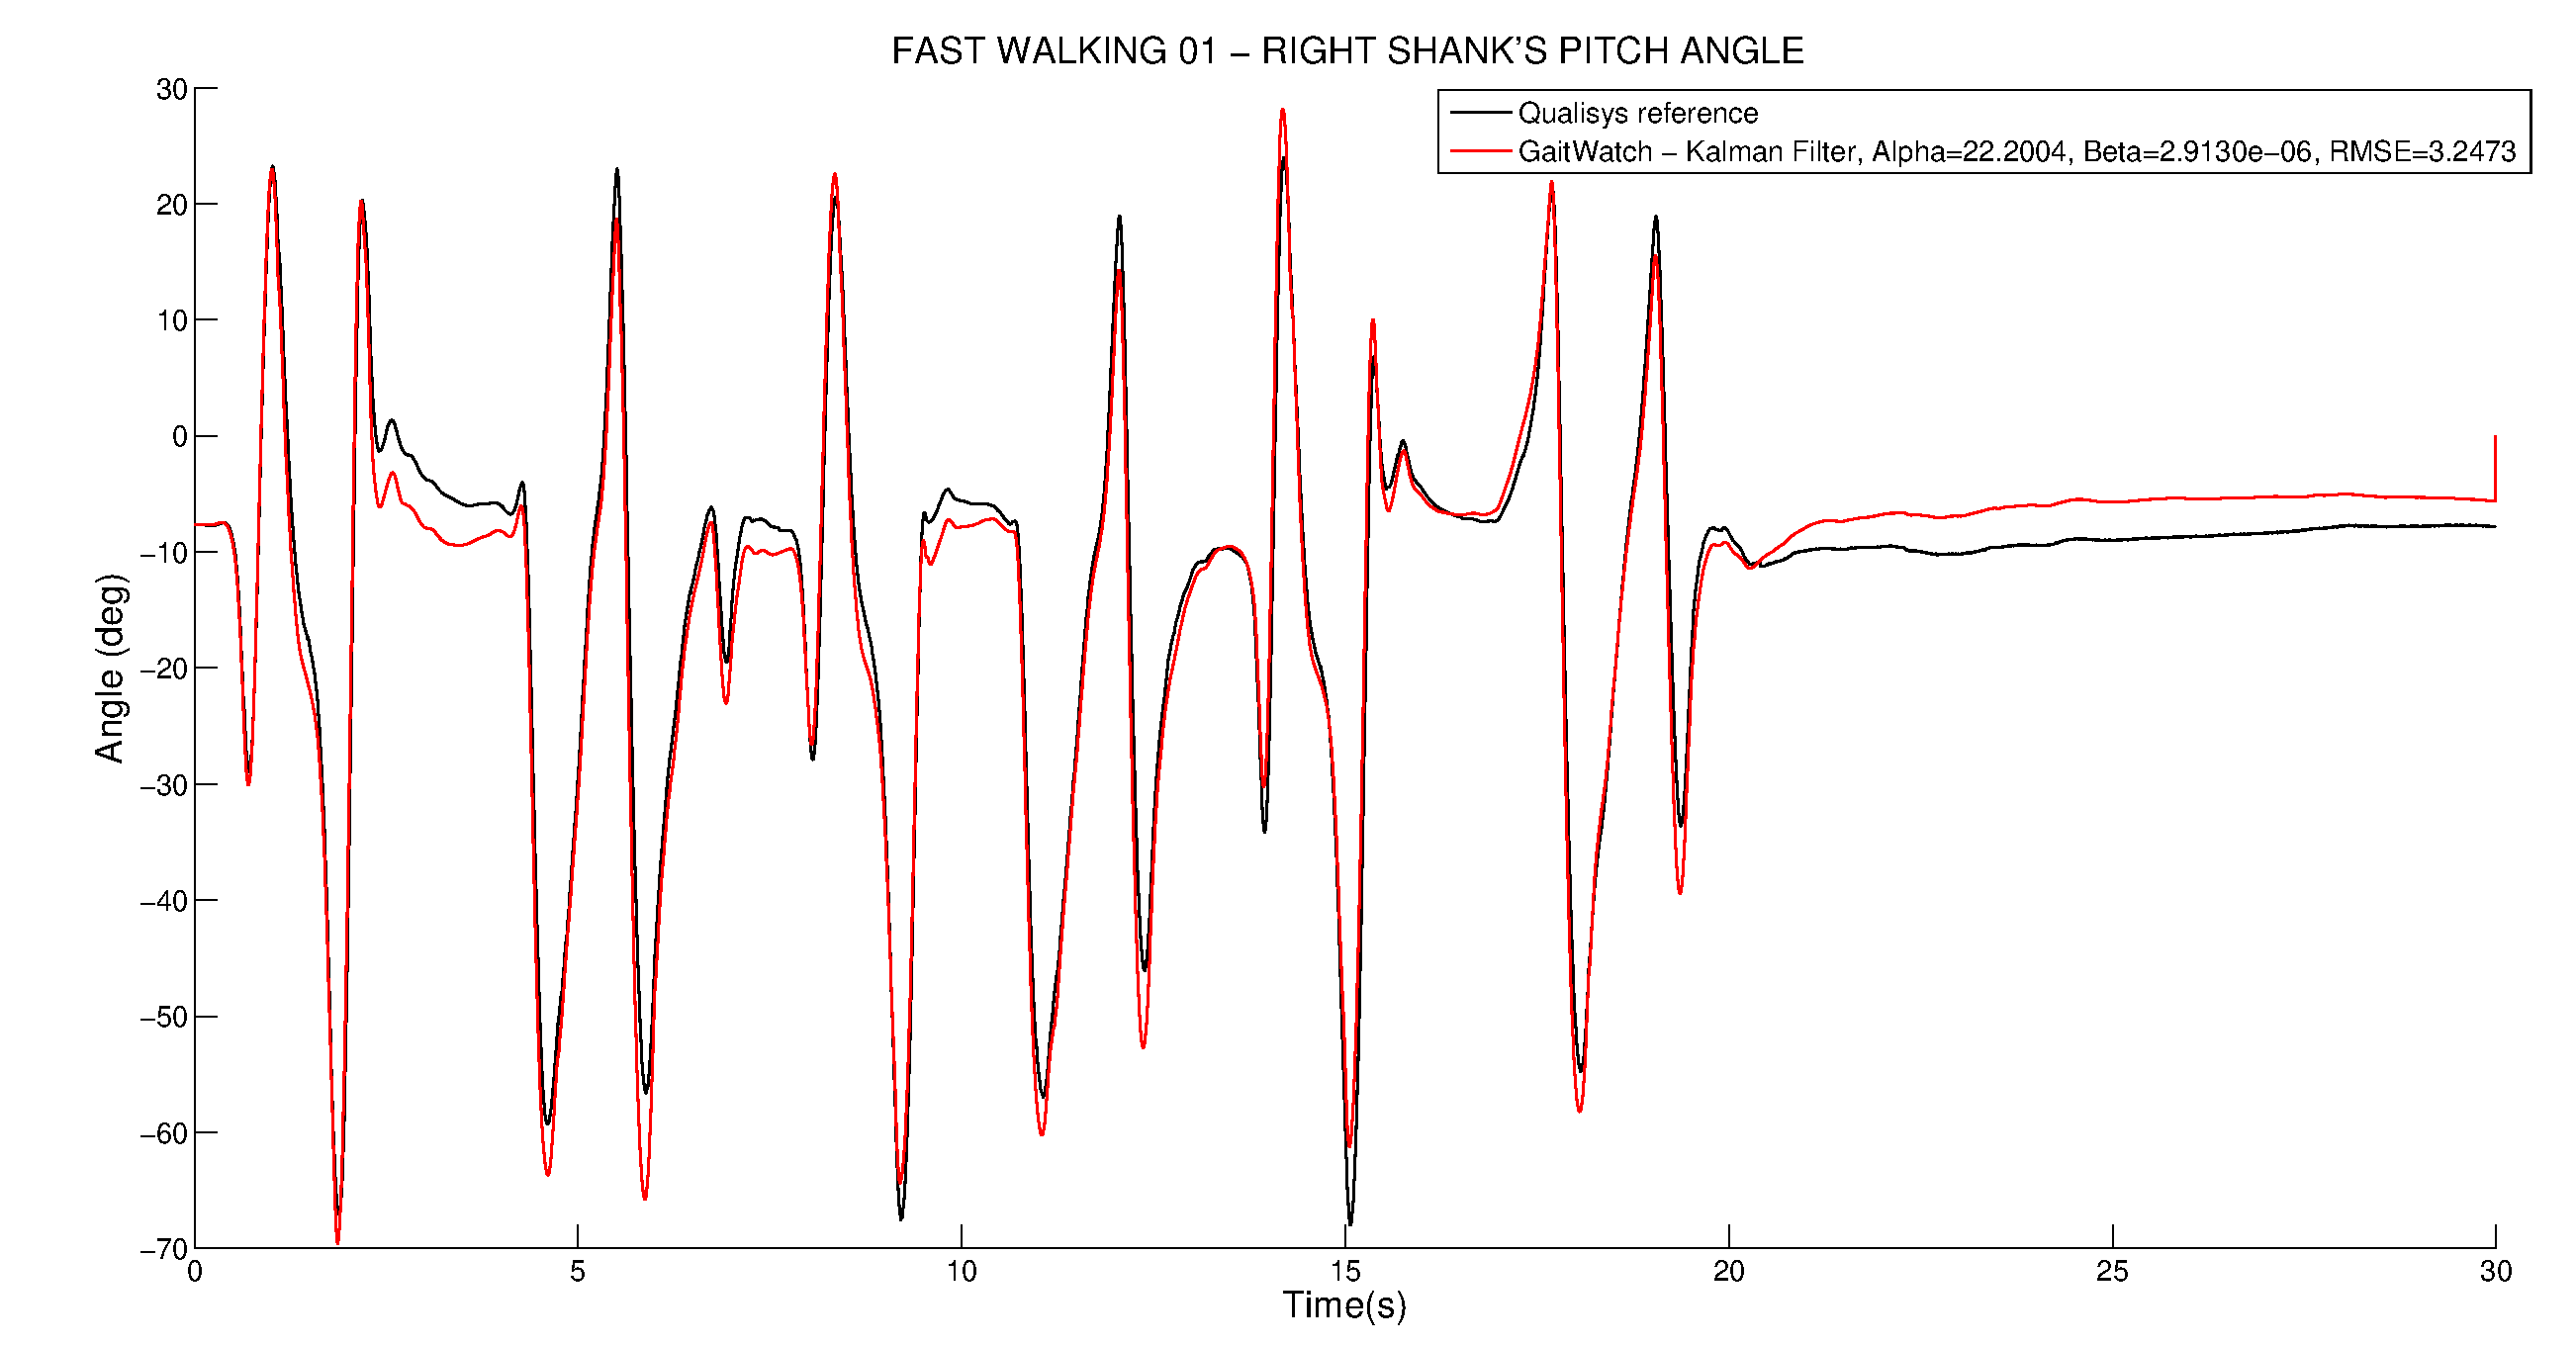
\includegraphics[width=1\textwidth]{figures/fast_walking_01_right_shank.eps}
\caption{Pitch angle of right shank measured while walking fast (GaitWatch vs. Qualisys).}
\label{fig:fast_walking_right_shank01}
\end{figure}

\begin{figure}[H]
\centering
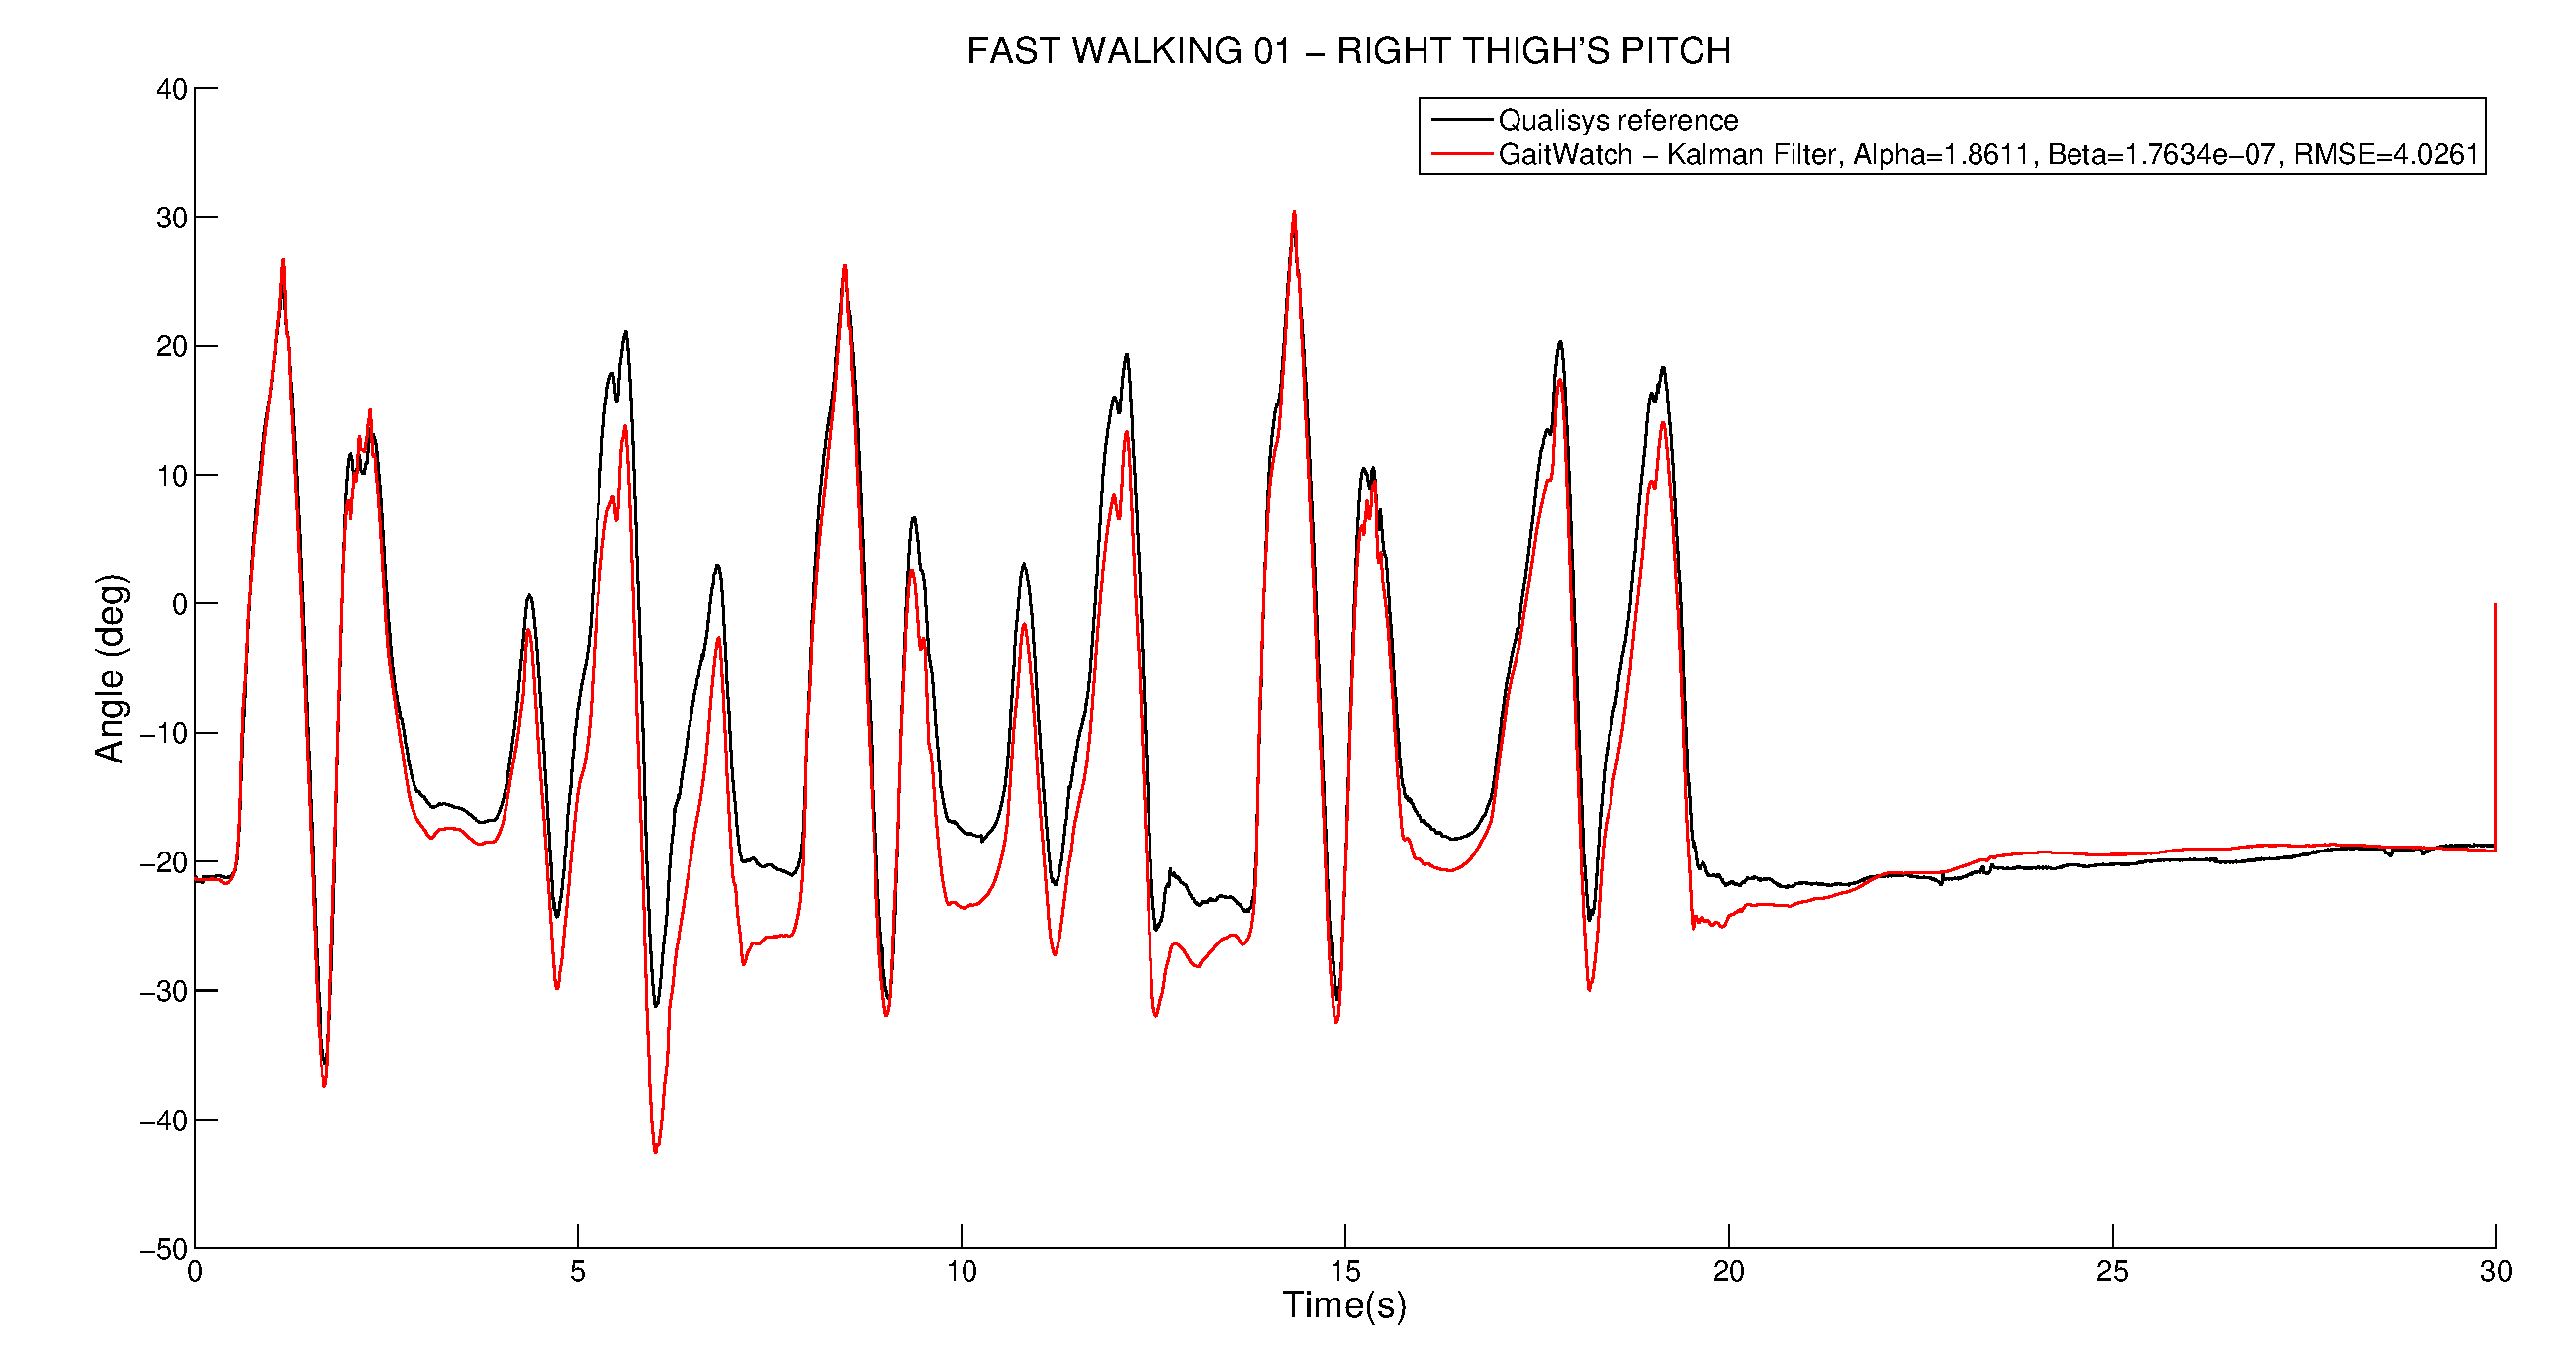
\includegraphics[width=1\textwidth]{figures/fast_walking_01_right_thigh.eps}
\caption{Pitch angle of right thigh measured while walking fast (GaitWatch vs. Qualisys).}
\label{fig:fast_walking_right_thigh01}
\end{figure}

\section{Jumping}

\begin{figure}[H]
\centering
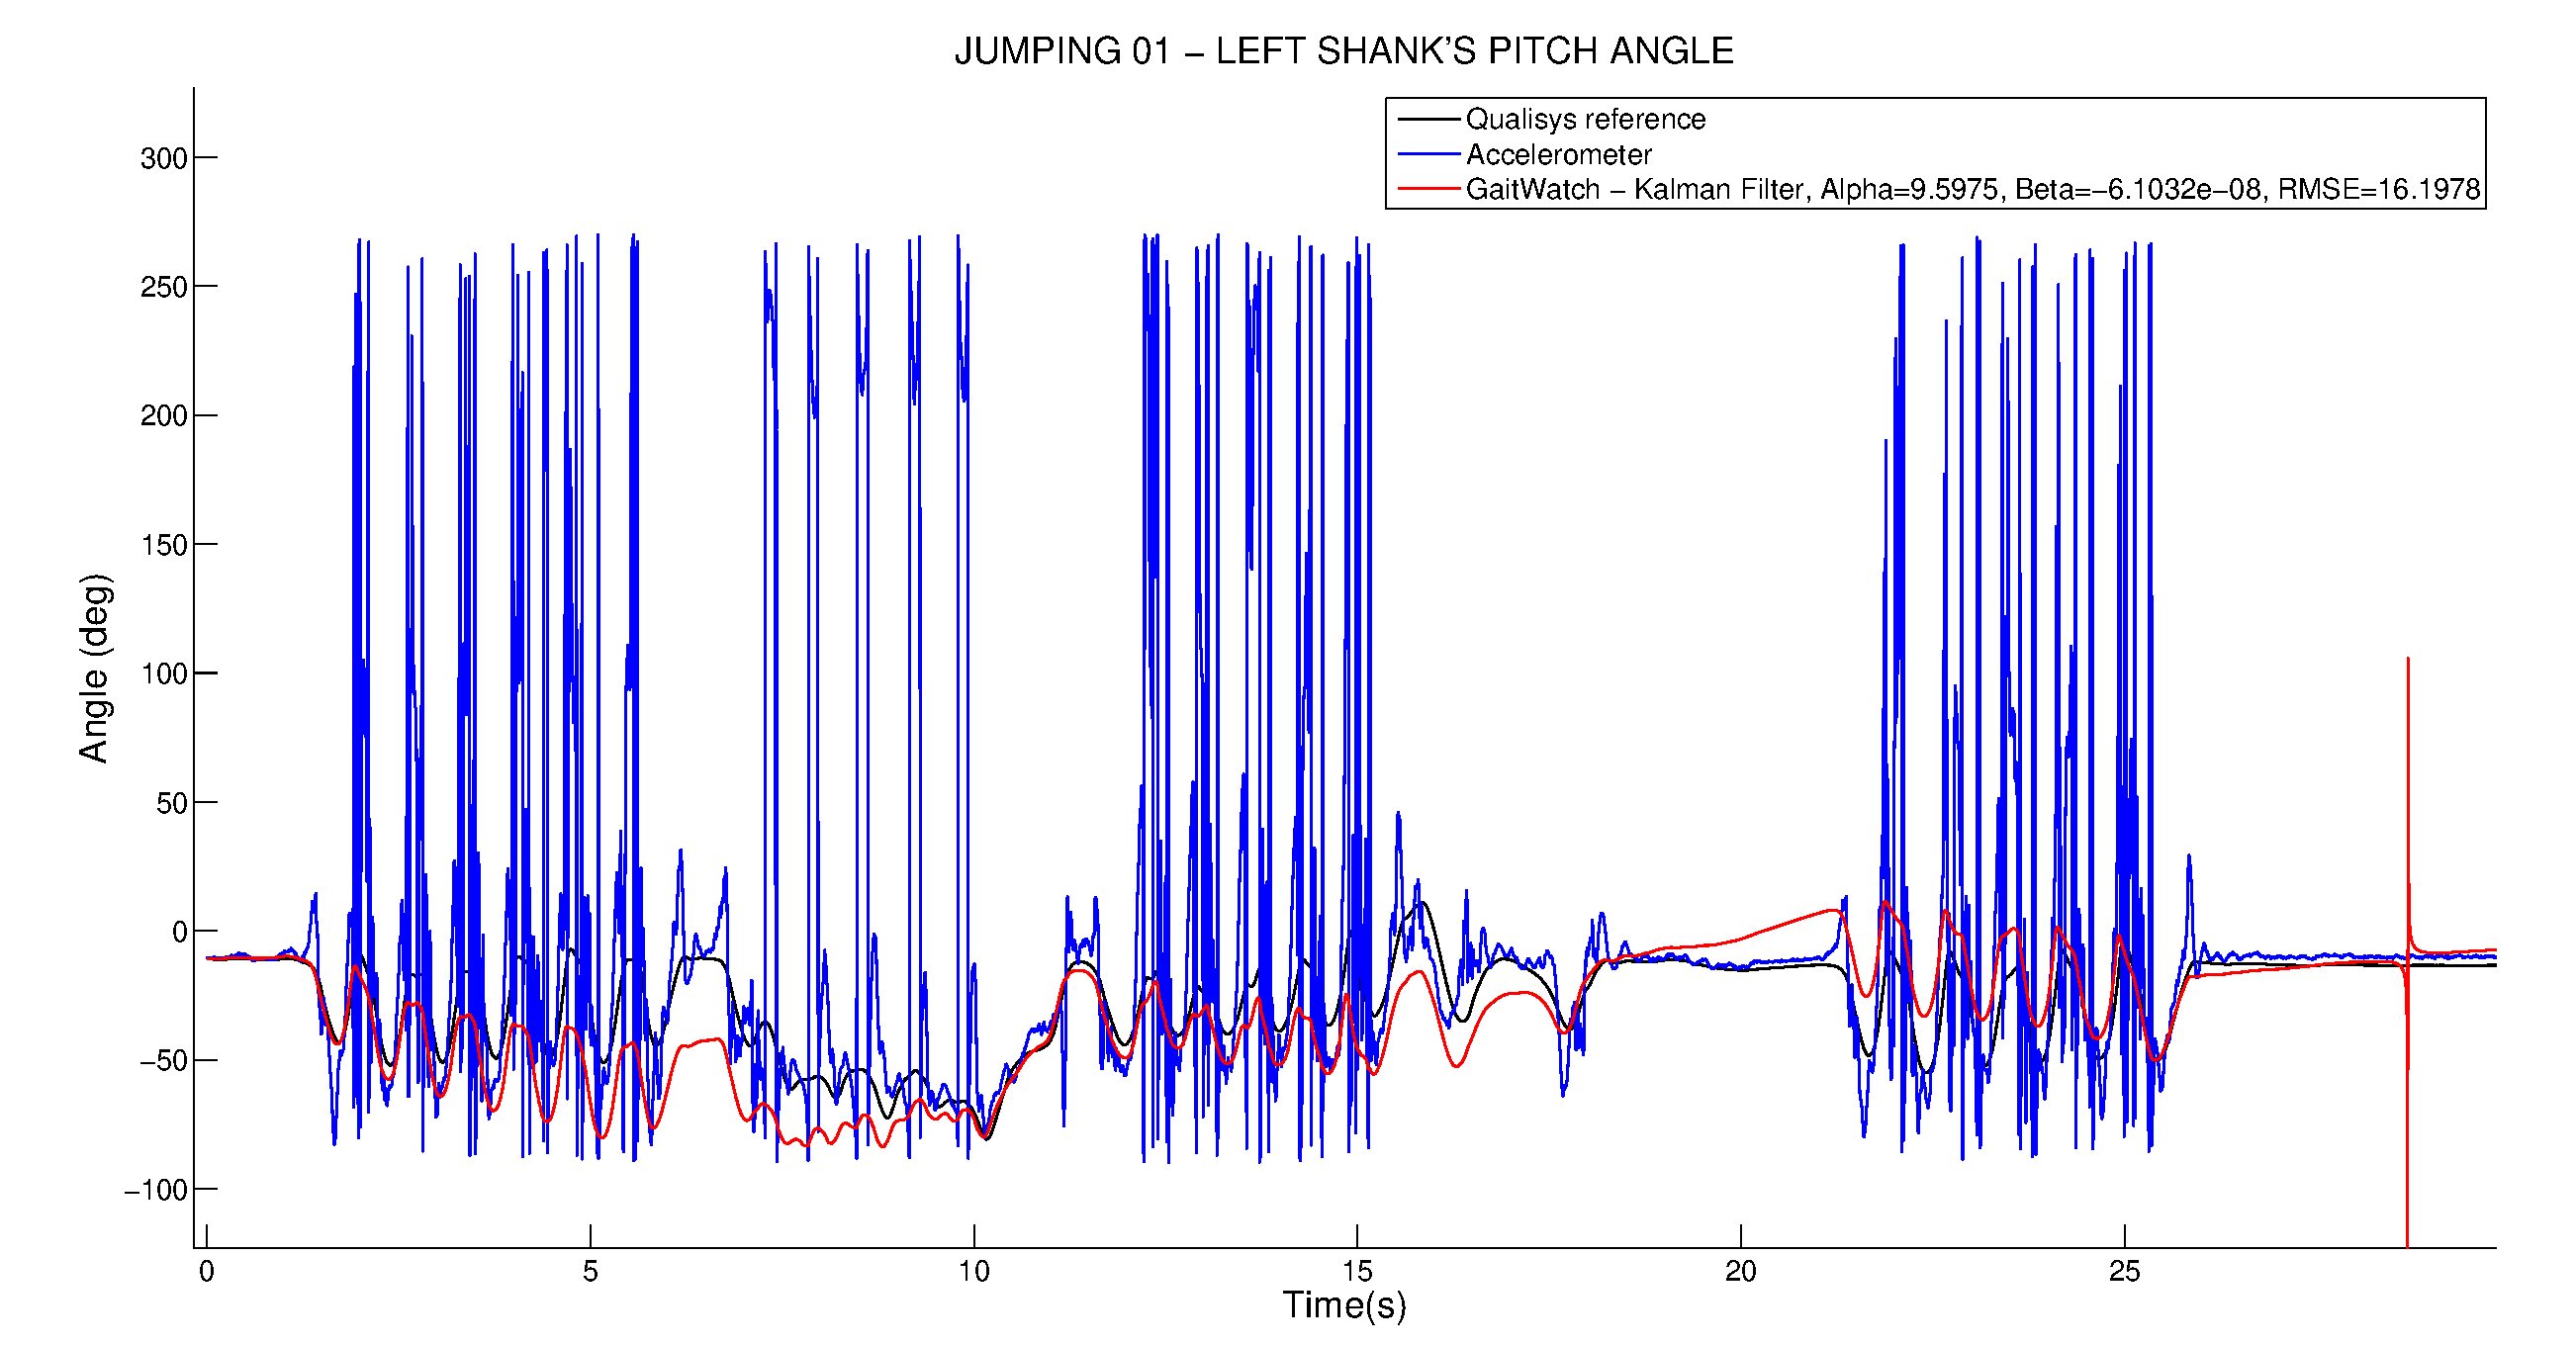
\includegraphics[width=1\textwidth]{figures/jumping_01_left_shank_with_acc.eps}
\caption{Pitch angle of left shank measured while jumping (GaitWatch vs. Qualisys).}
\label{fig:jumping_left_shank01}
\end{figure}

\begin{figure}[H]
\centering
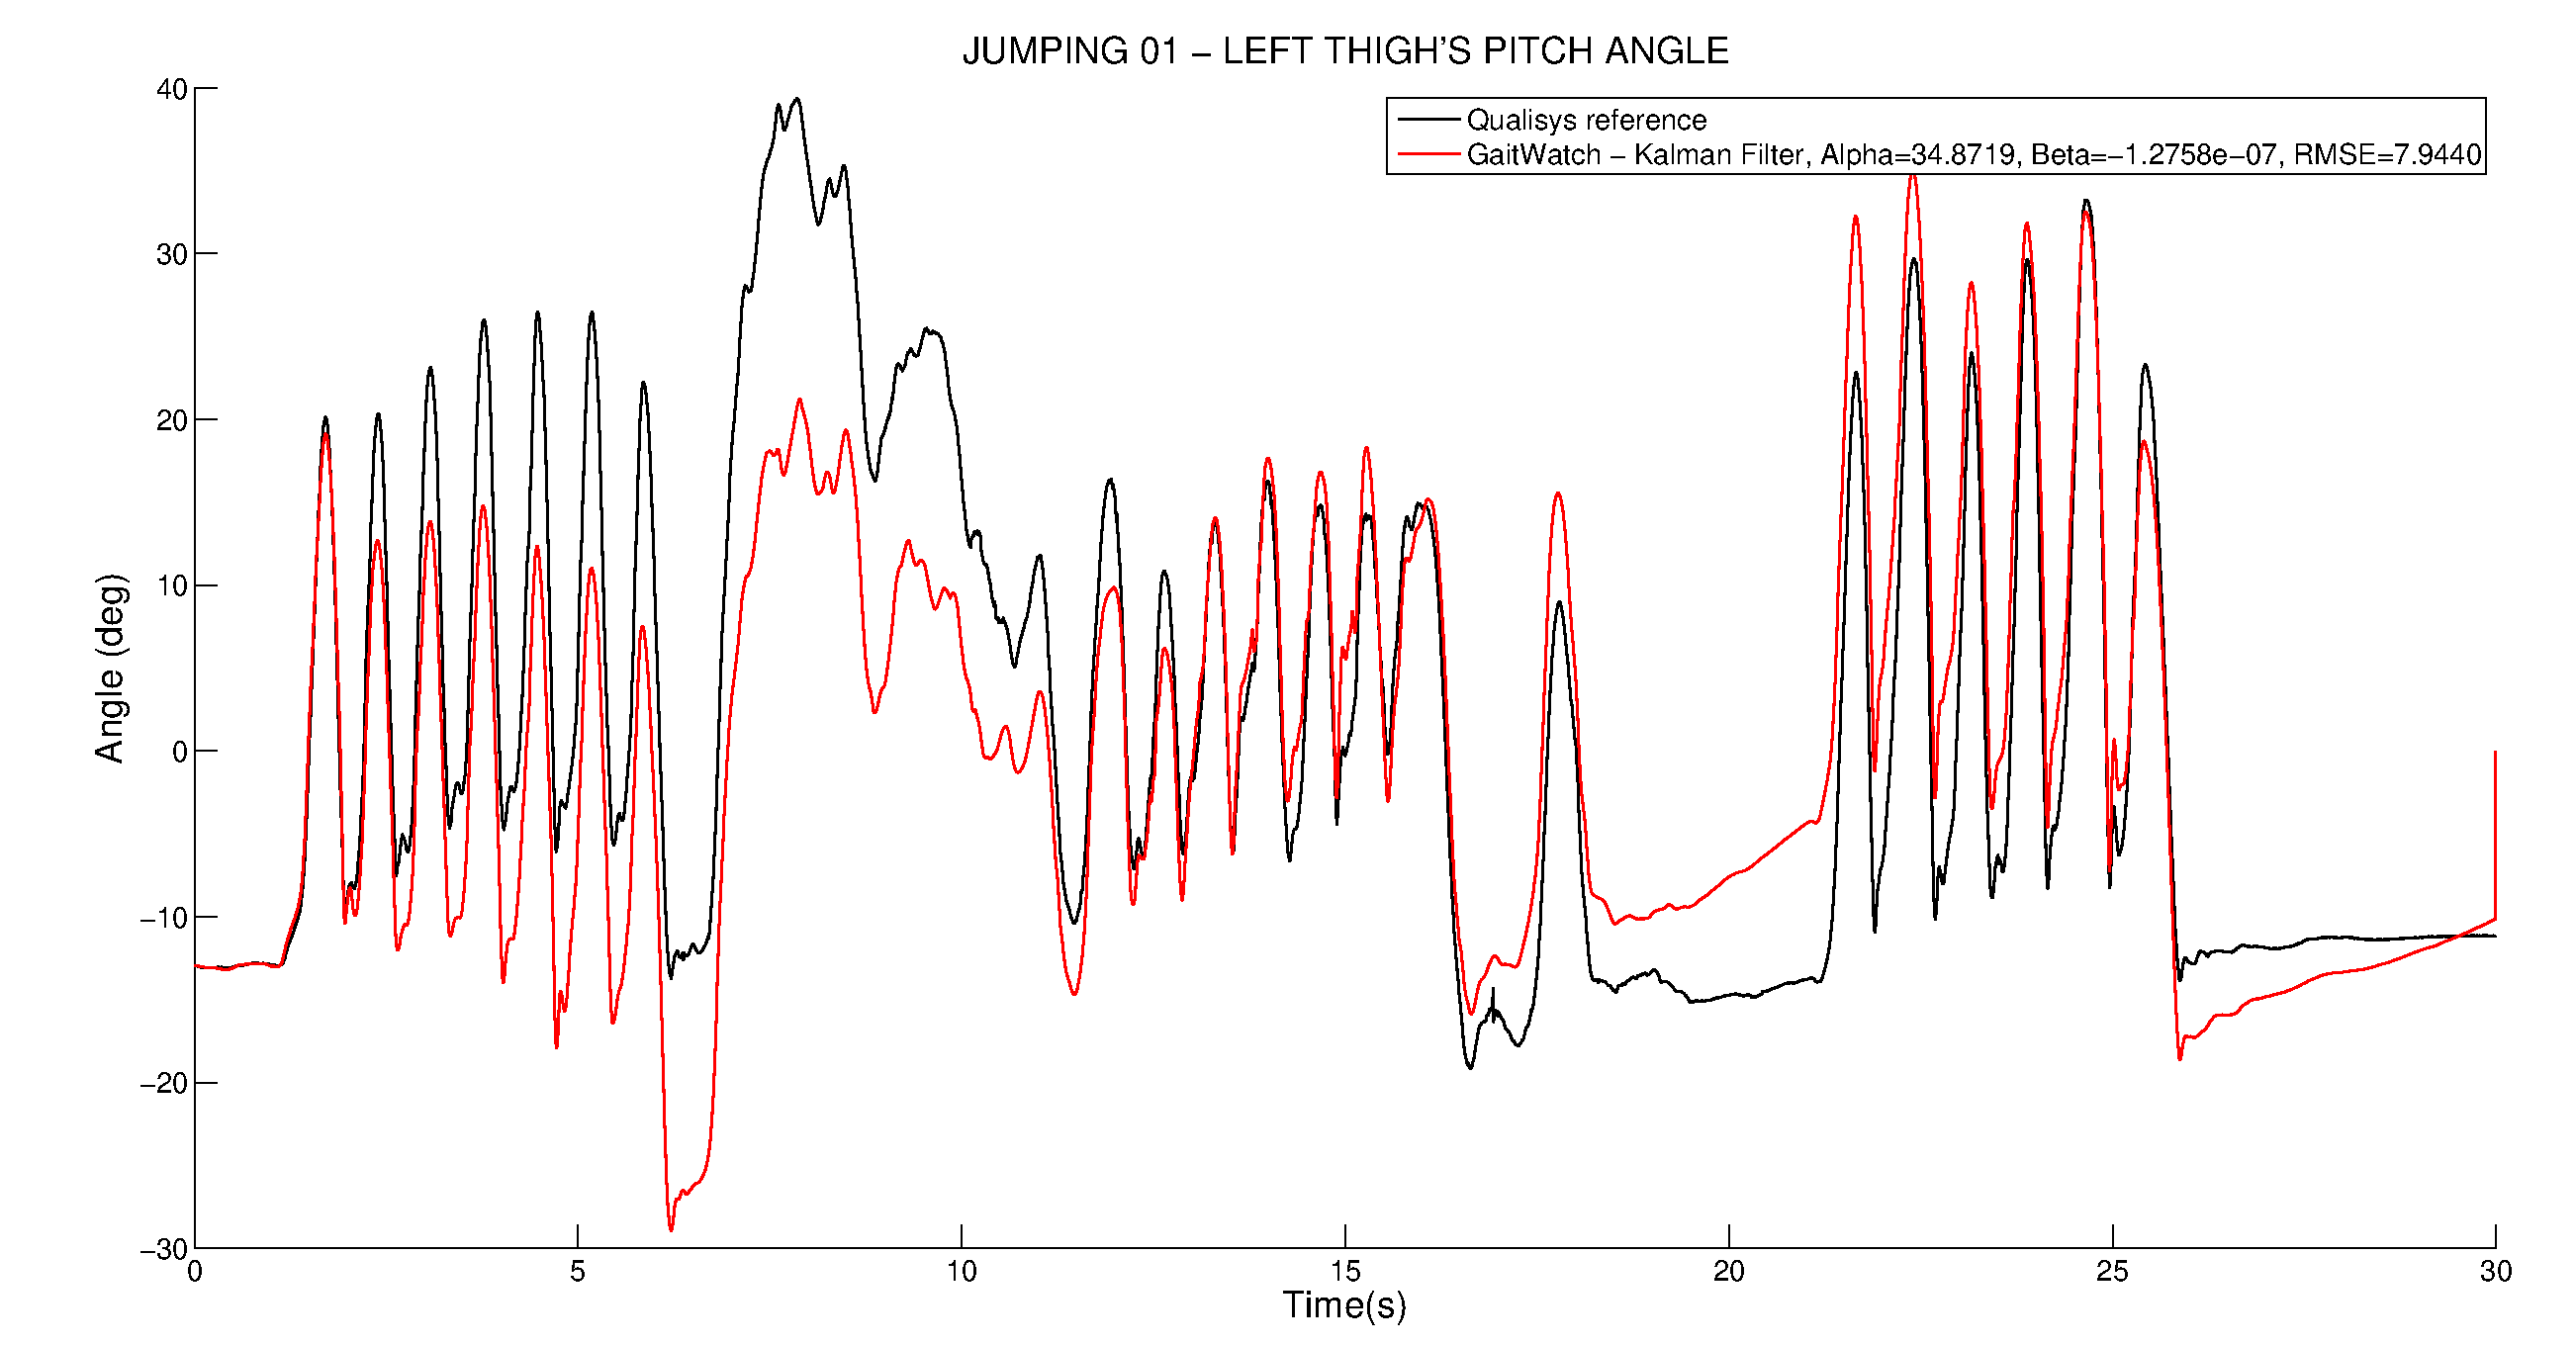
\includegraphics[width=1\textwidth]{figures/jumping_01_left_thigh.eps}
\caption{Pitch angle of left thigh measured while jumping (GaitWatch vs. Qualisys).}
\label{fig:jumping_left_thigh01}
\end{figure}

\begin{figure}[H]
\centering
\includegraphics[width=1\textwidth]{figures/jumping_01_right_shank.eps}
\caption{Pitch angle of right shank measured while jumping (GaitWatch vs. Qualisys).}
\label{fig:jumping_right_shank01}
\end{figure}

\begin{figure}[H]
\centering
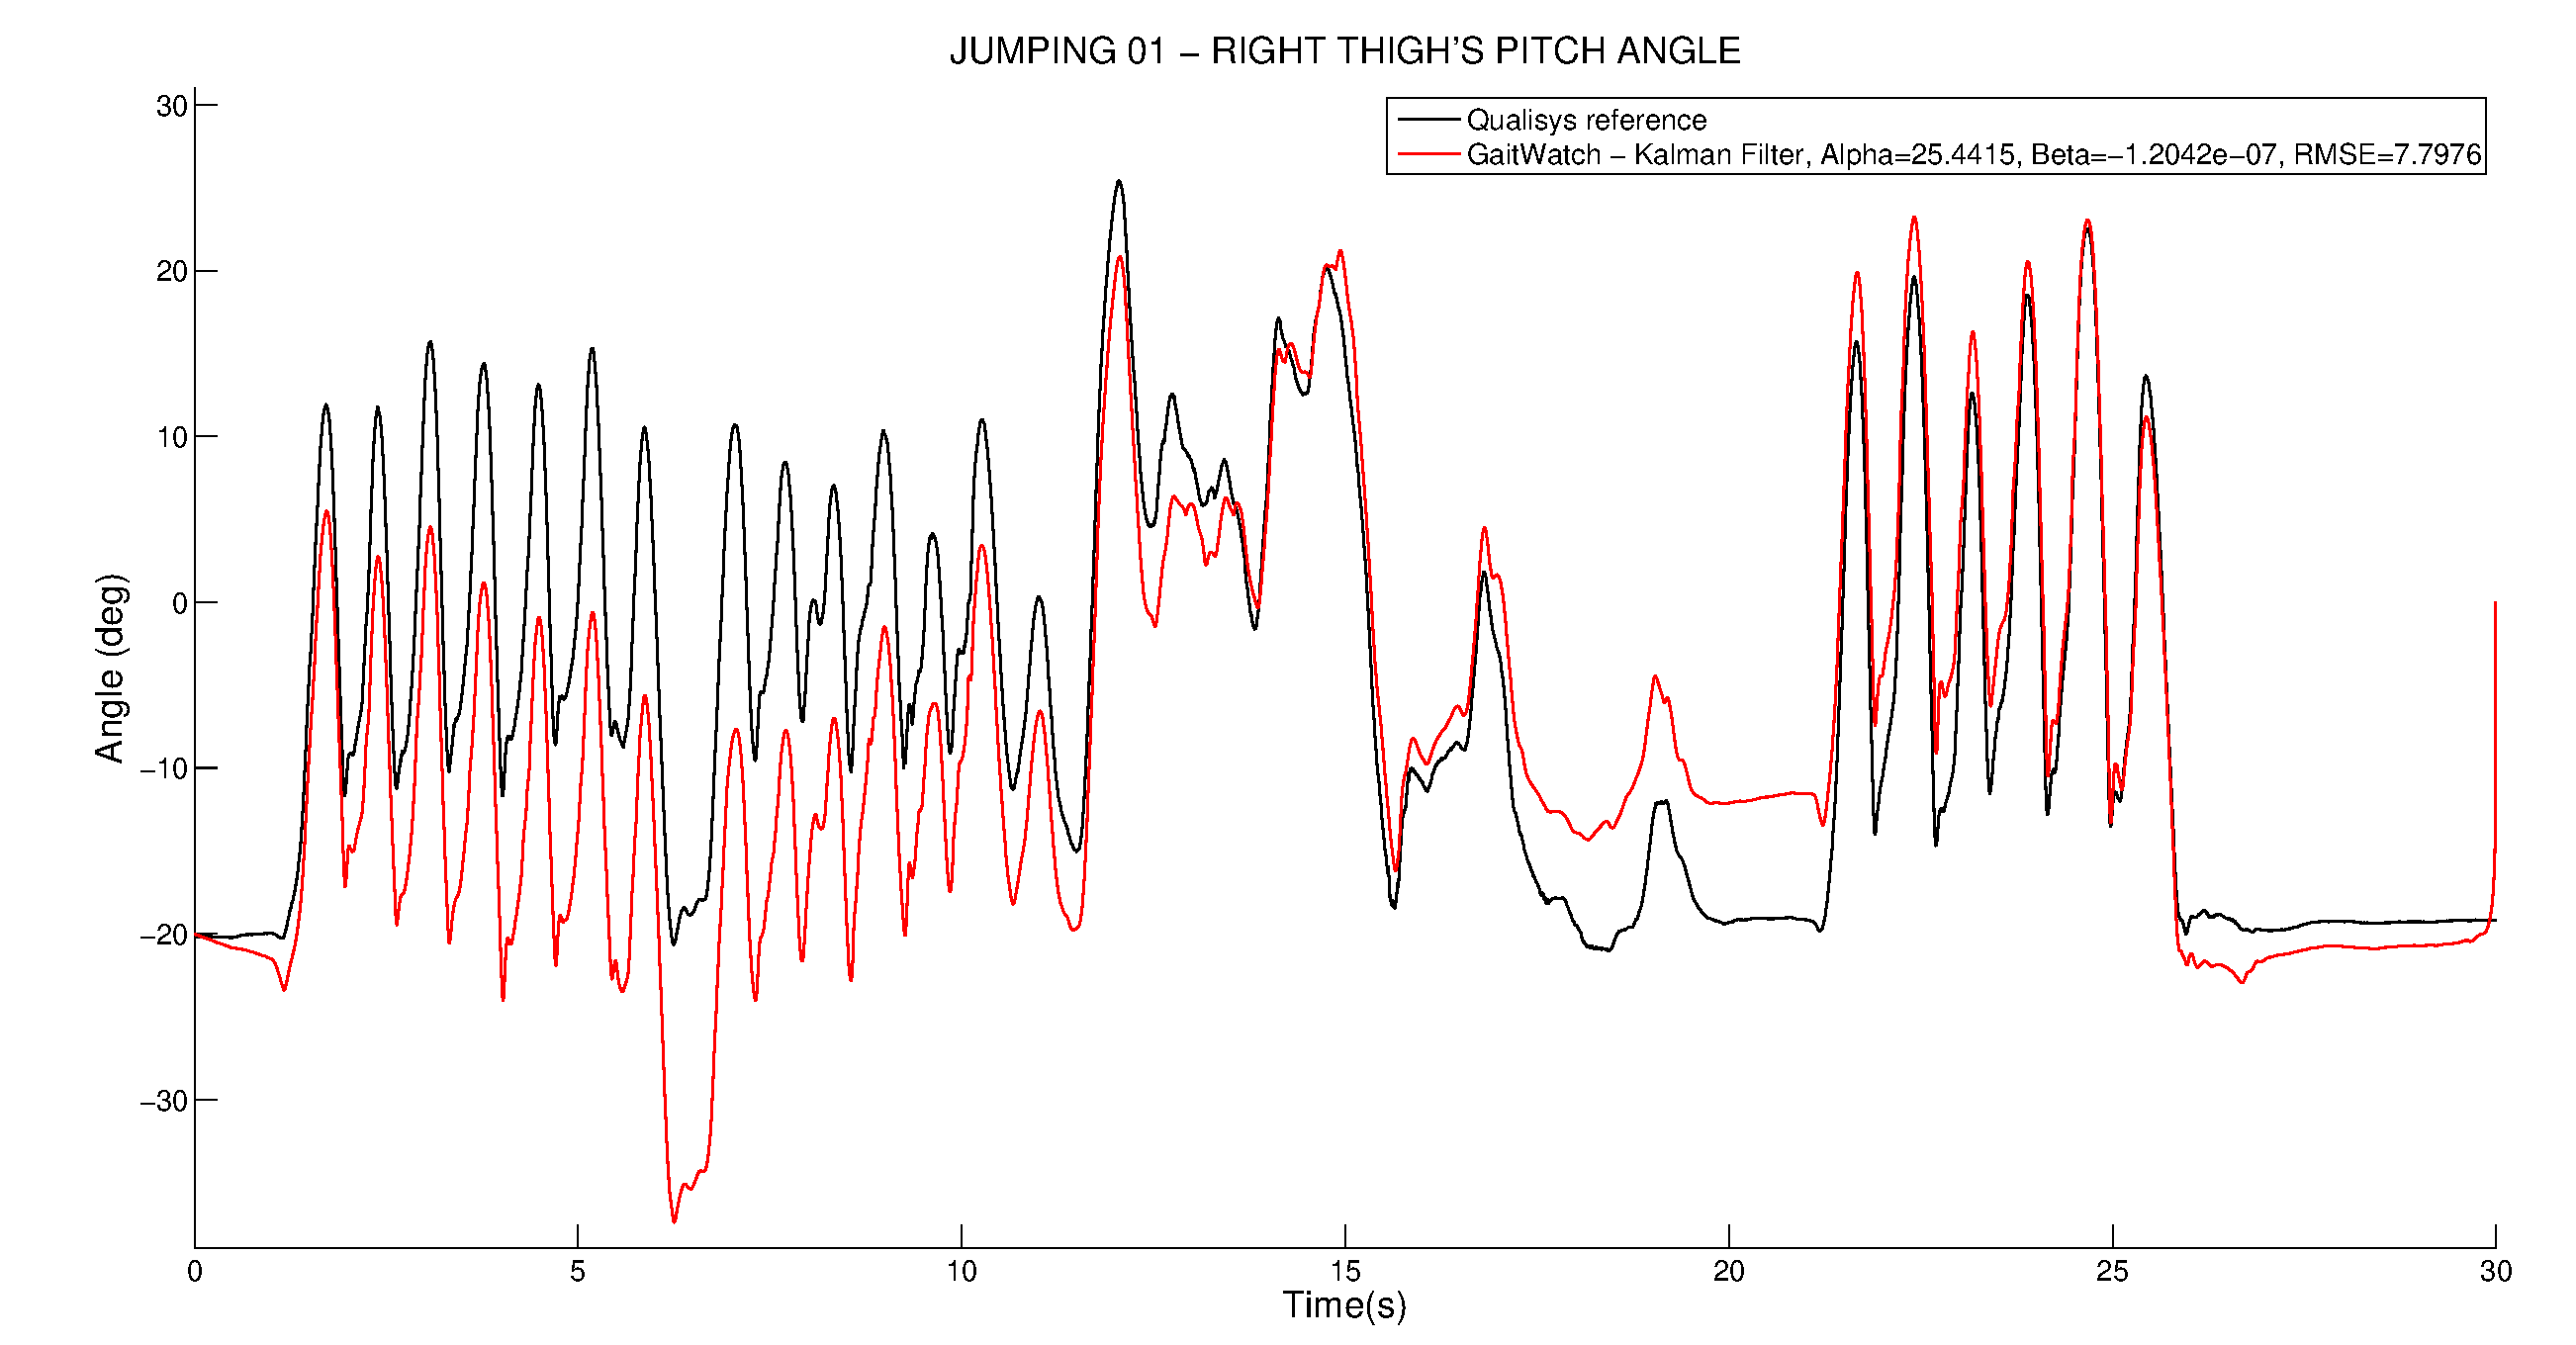
\includegraphics[width=1\textwidth]{figures/jumping_01_right_thigh.eps}
\caption{Pitch angle of right thigh measured while jumping (GaitWatch vs. Qualisys).}
\label{fig:jumping_right_thigh01}
\end{figure}

\section{Leg motion}

\begin{figure}[H]
\centering
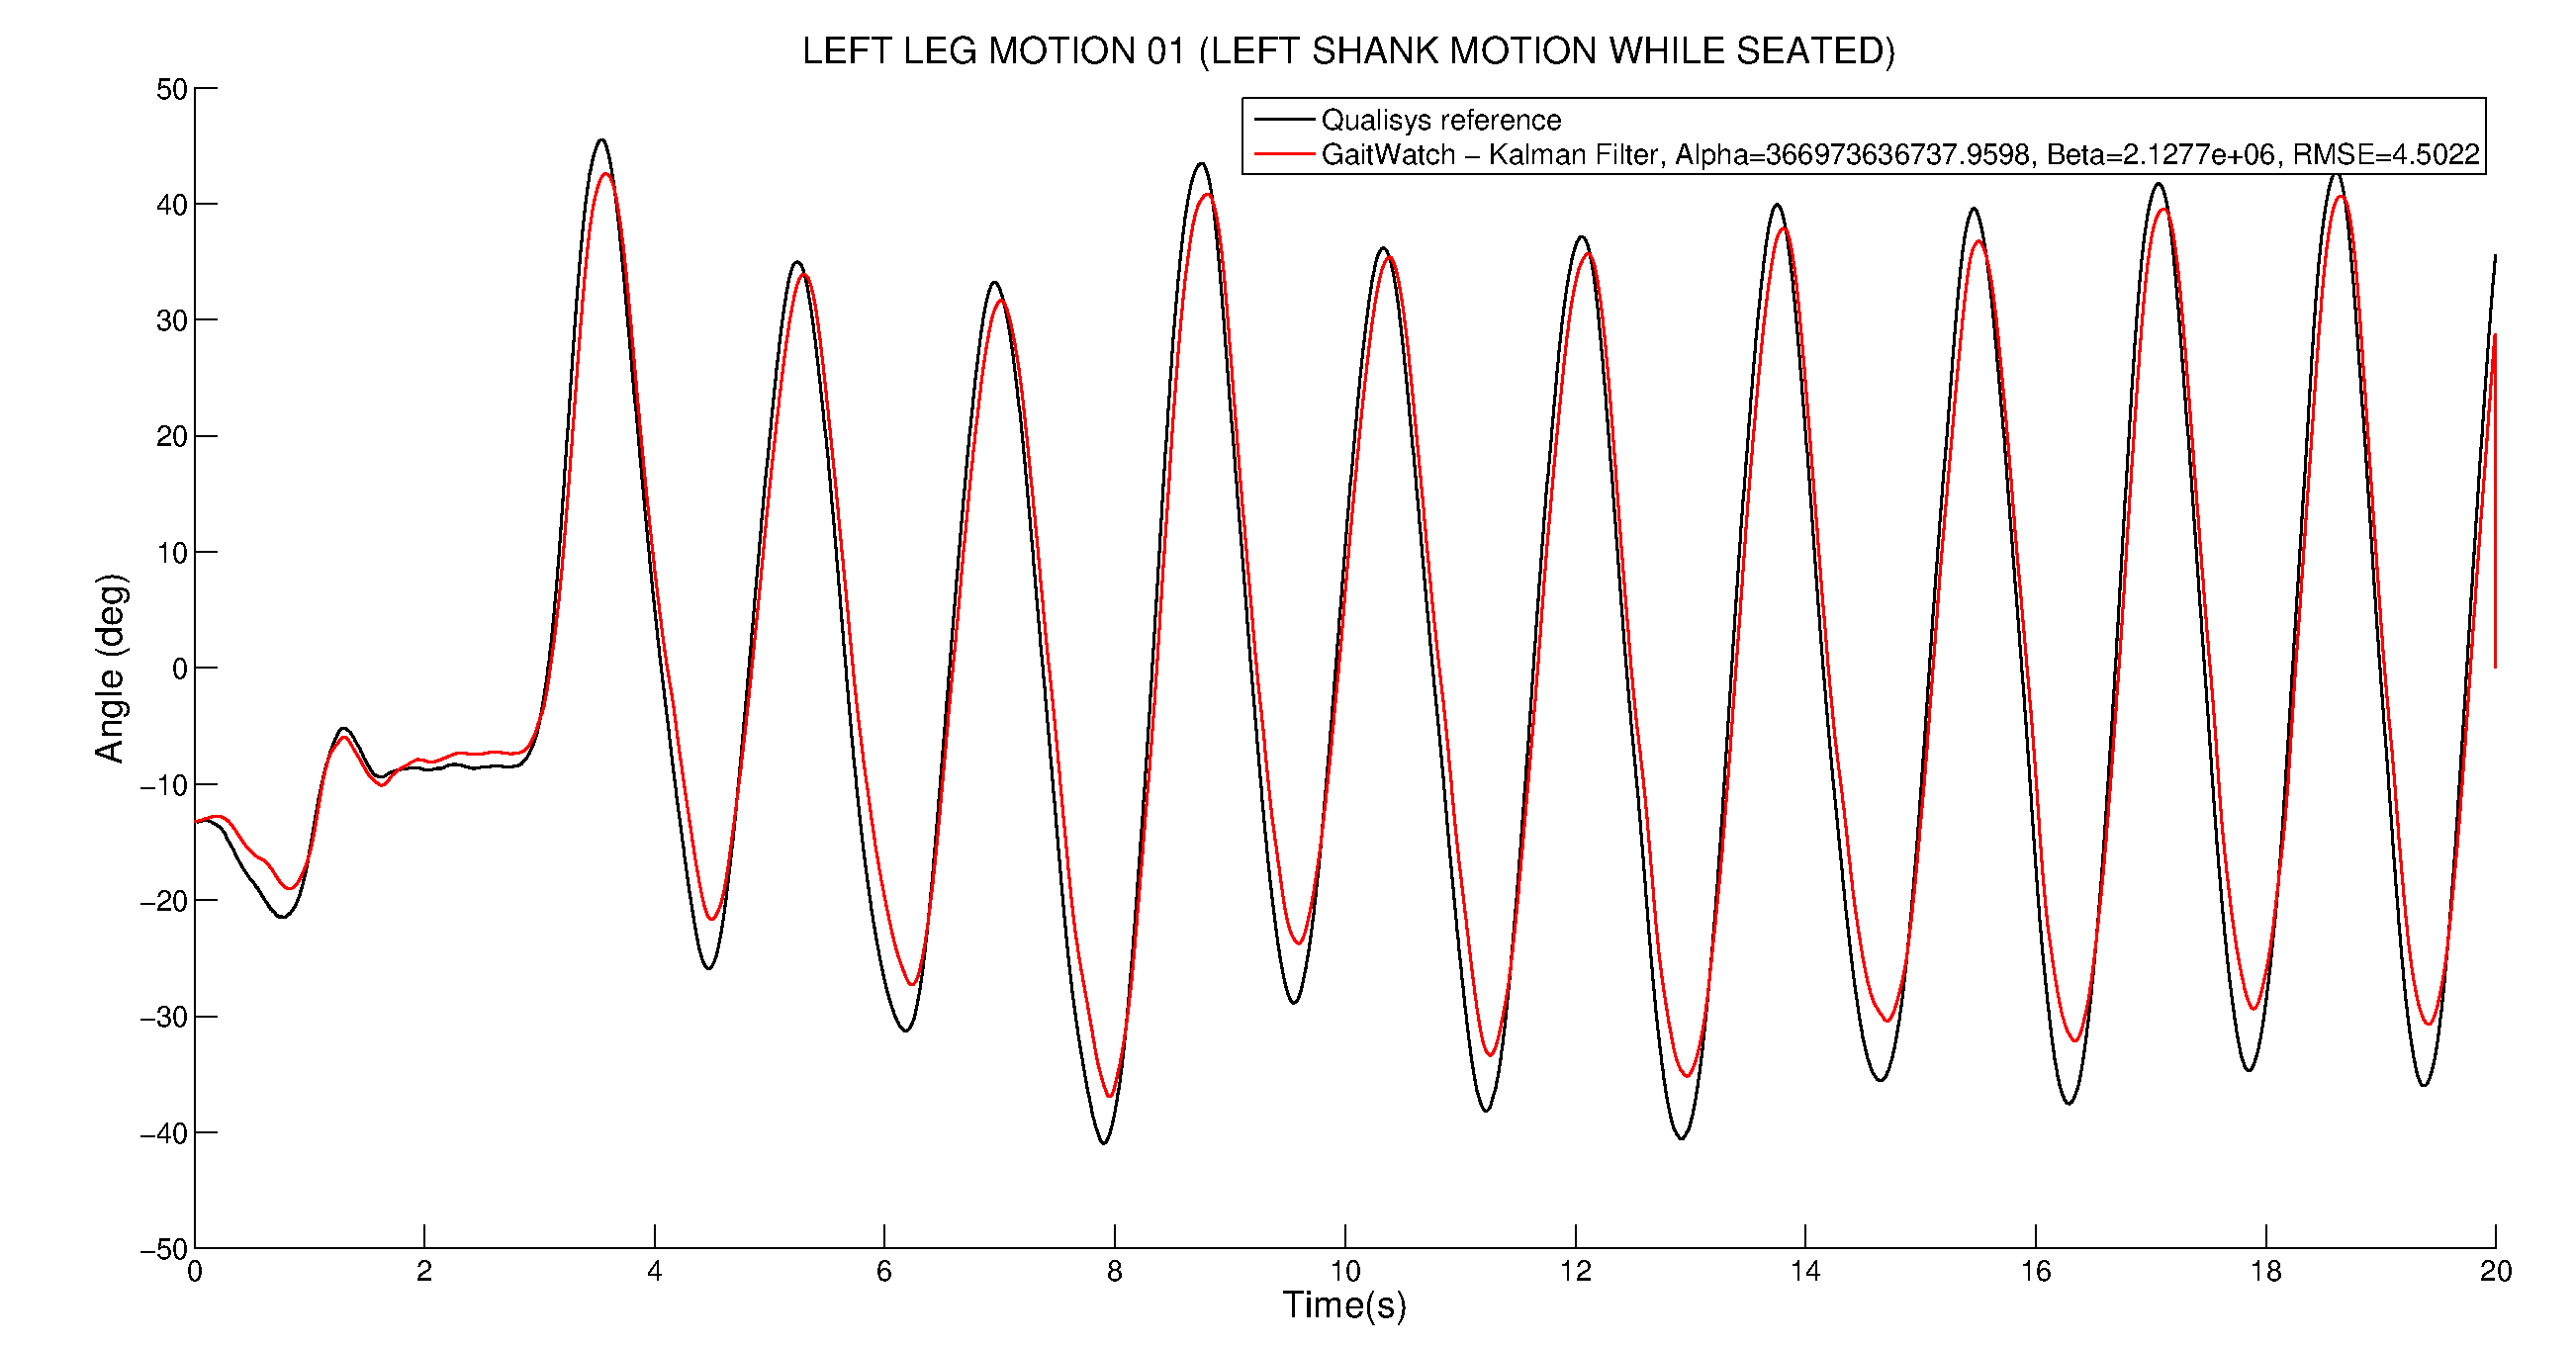
\includegraphics[width=1\textwidth]{figures/Left_leg_motion_01_shank.eps}
\caption{Pitch angle while swinging left shank. (GaitWatch vs. Qualisys).}
\label{fig:Left_leg_motion_01_shank}
\end{figure}

\begin{figure}[H]
\centering
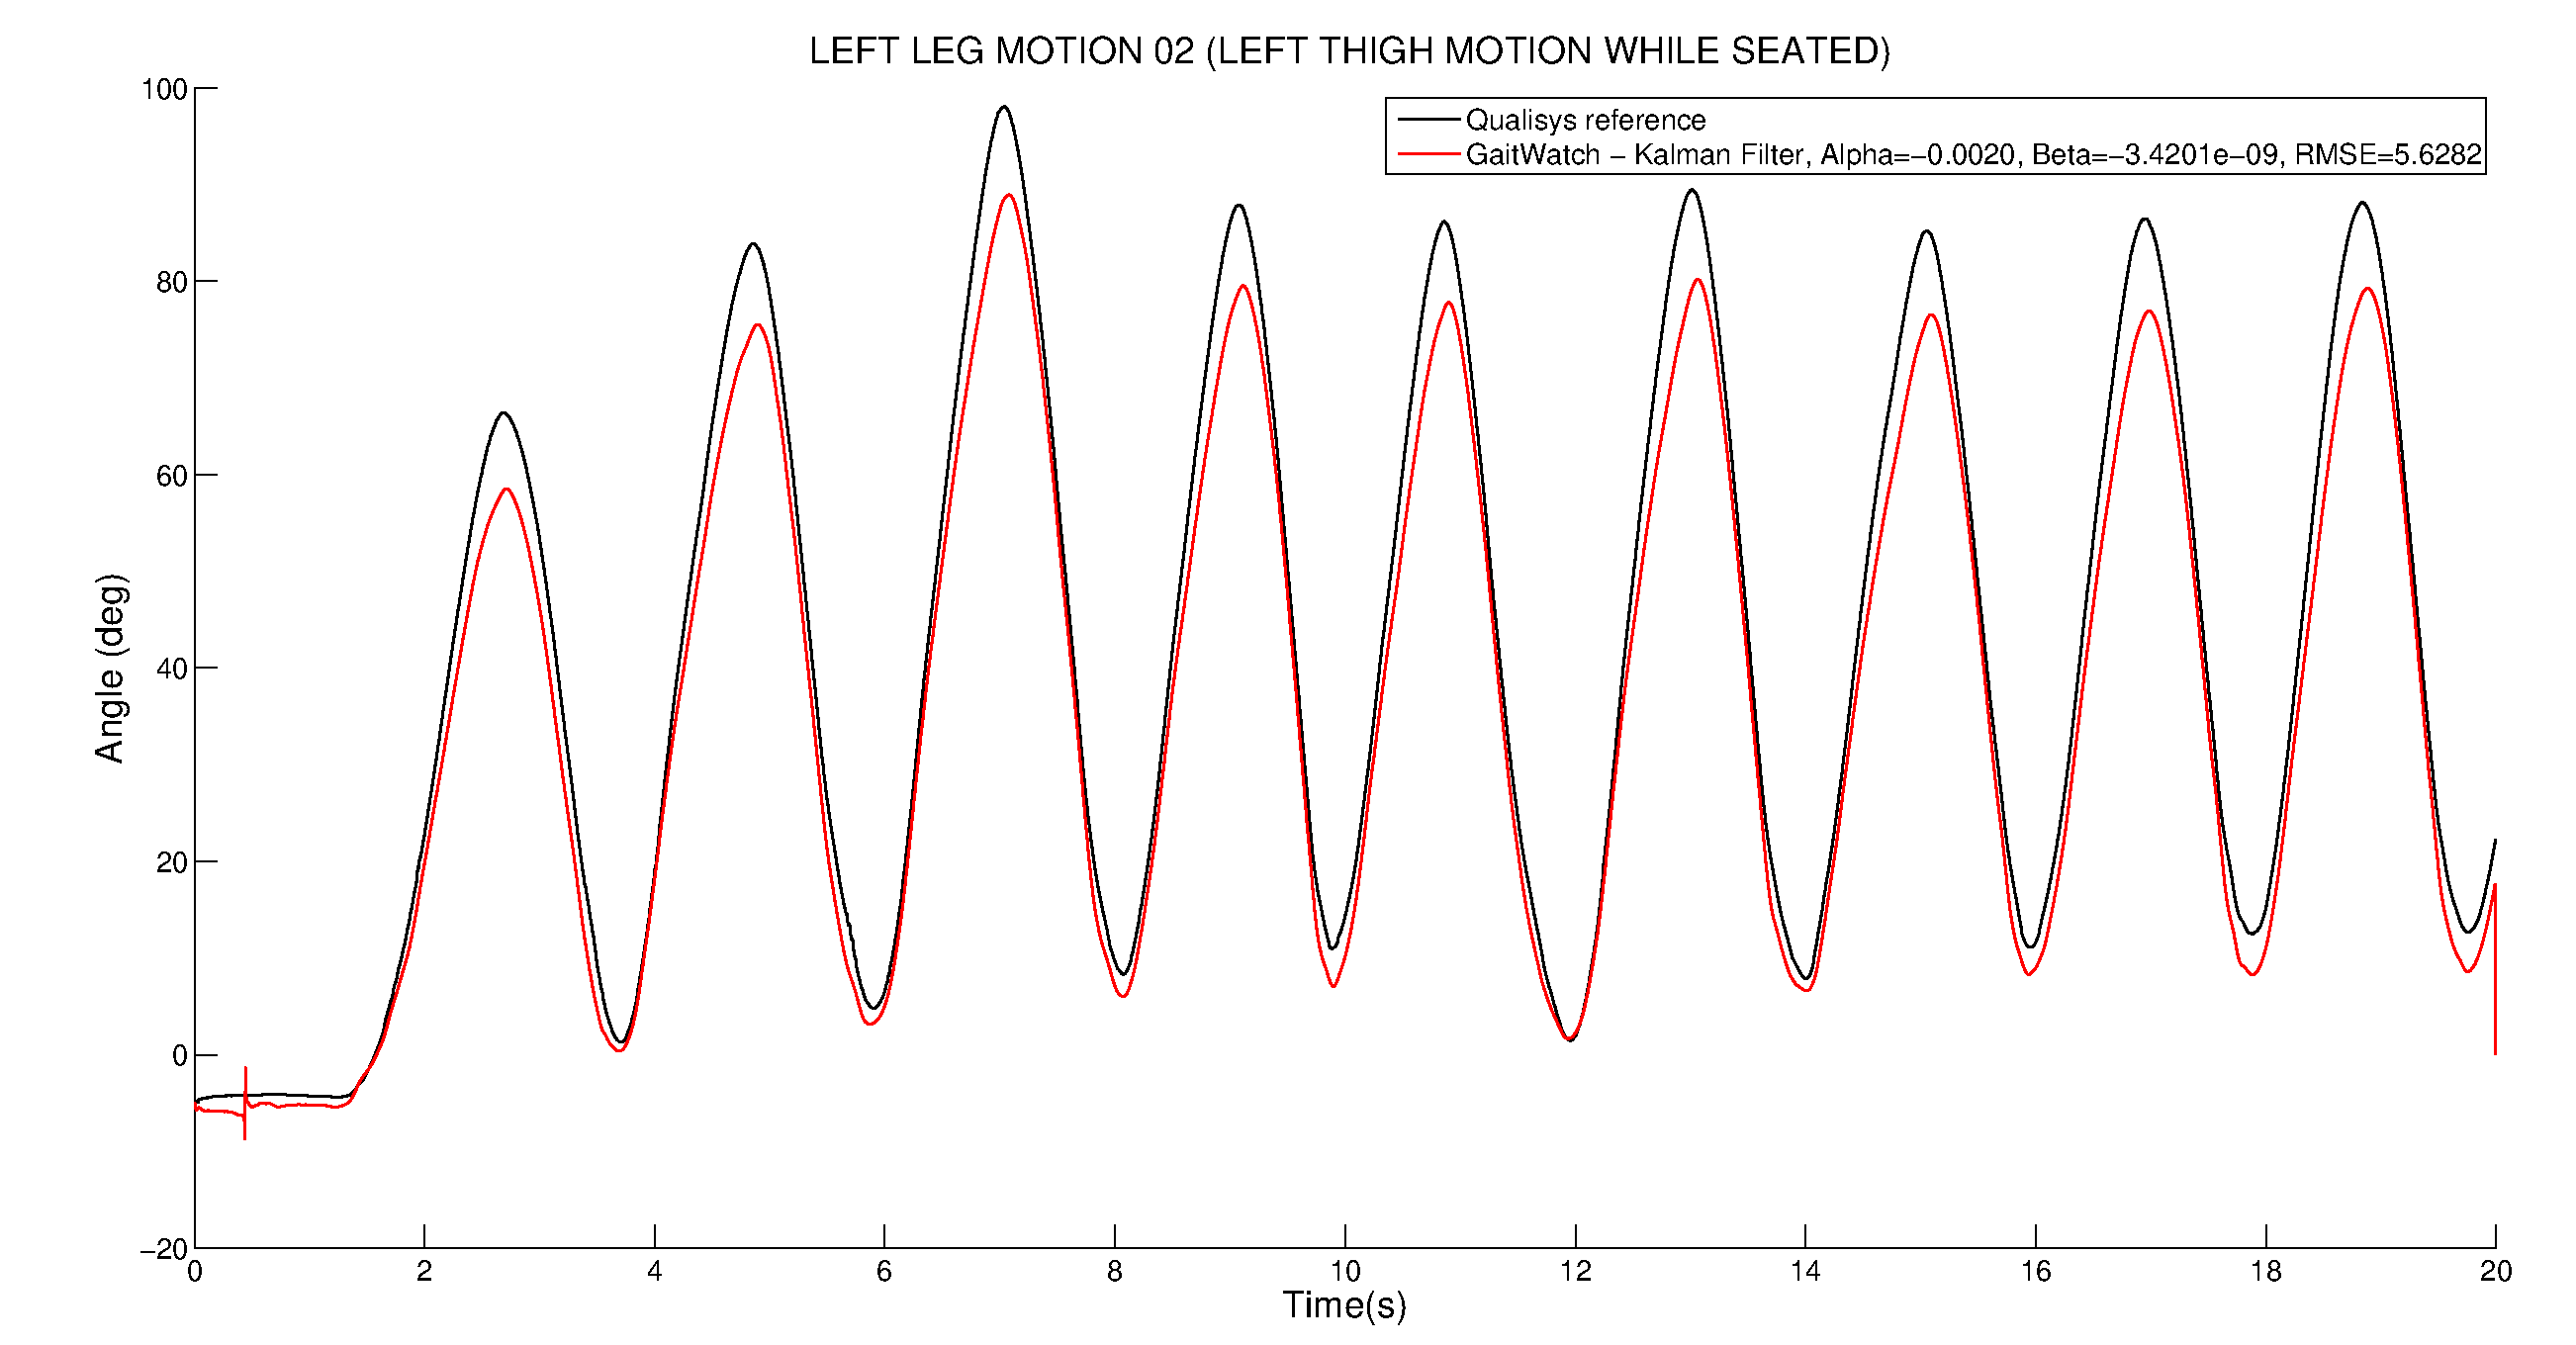
\includegraphics[width=1\textwidth]{figures/Left_leg_motion_02_thigh.eps}
\caption{Pitch angle while swinging left thigh. (GaitWatch vs. Qualisys).}
\label{fig:Left_leg_motion_02_thigh}
\end{figure}

\begin{figure}[H]
\centering
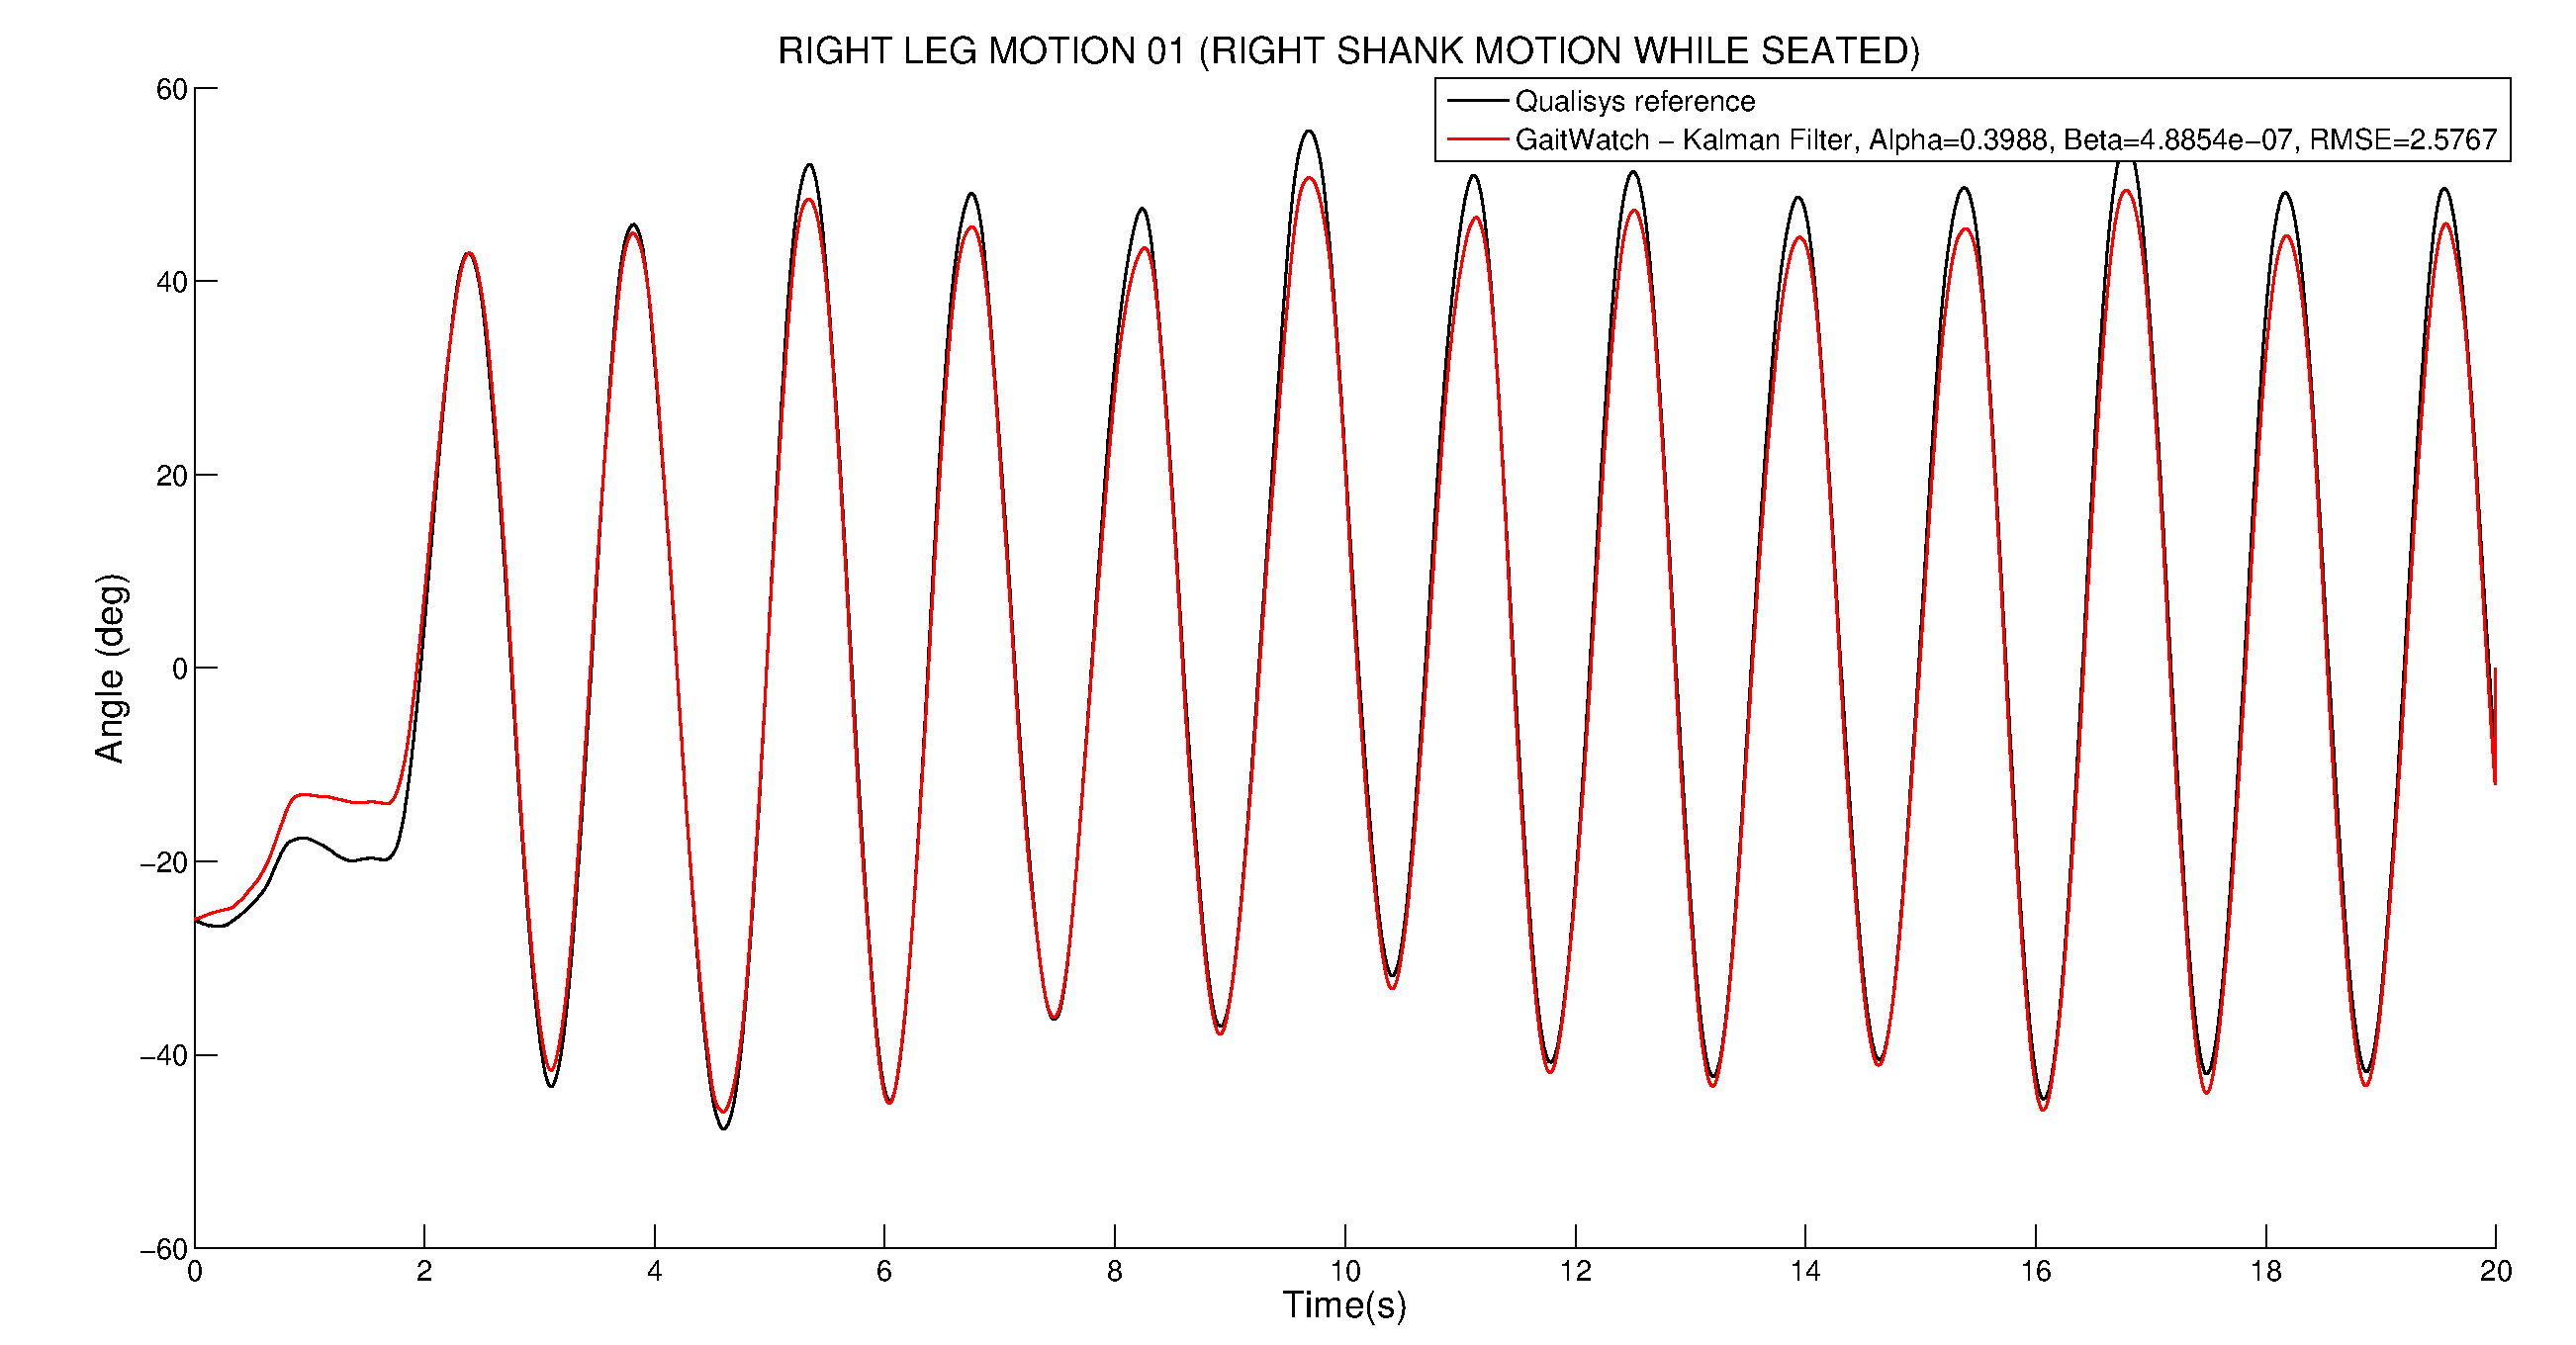
\includegraphics[width=1\textwidth]{figures/Right_leg_motion_01_shank.eps}
\caption{Pitch angle while swinging right shank. (GaitWatch vs. Qualisys).}
\label{fig:Right_leg_motion_01_shank}
\end{figure}

\begin{figure}[H]
\centering
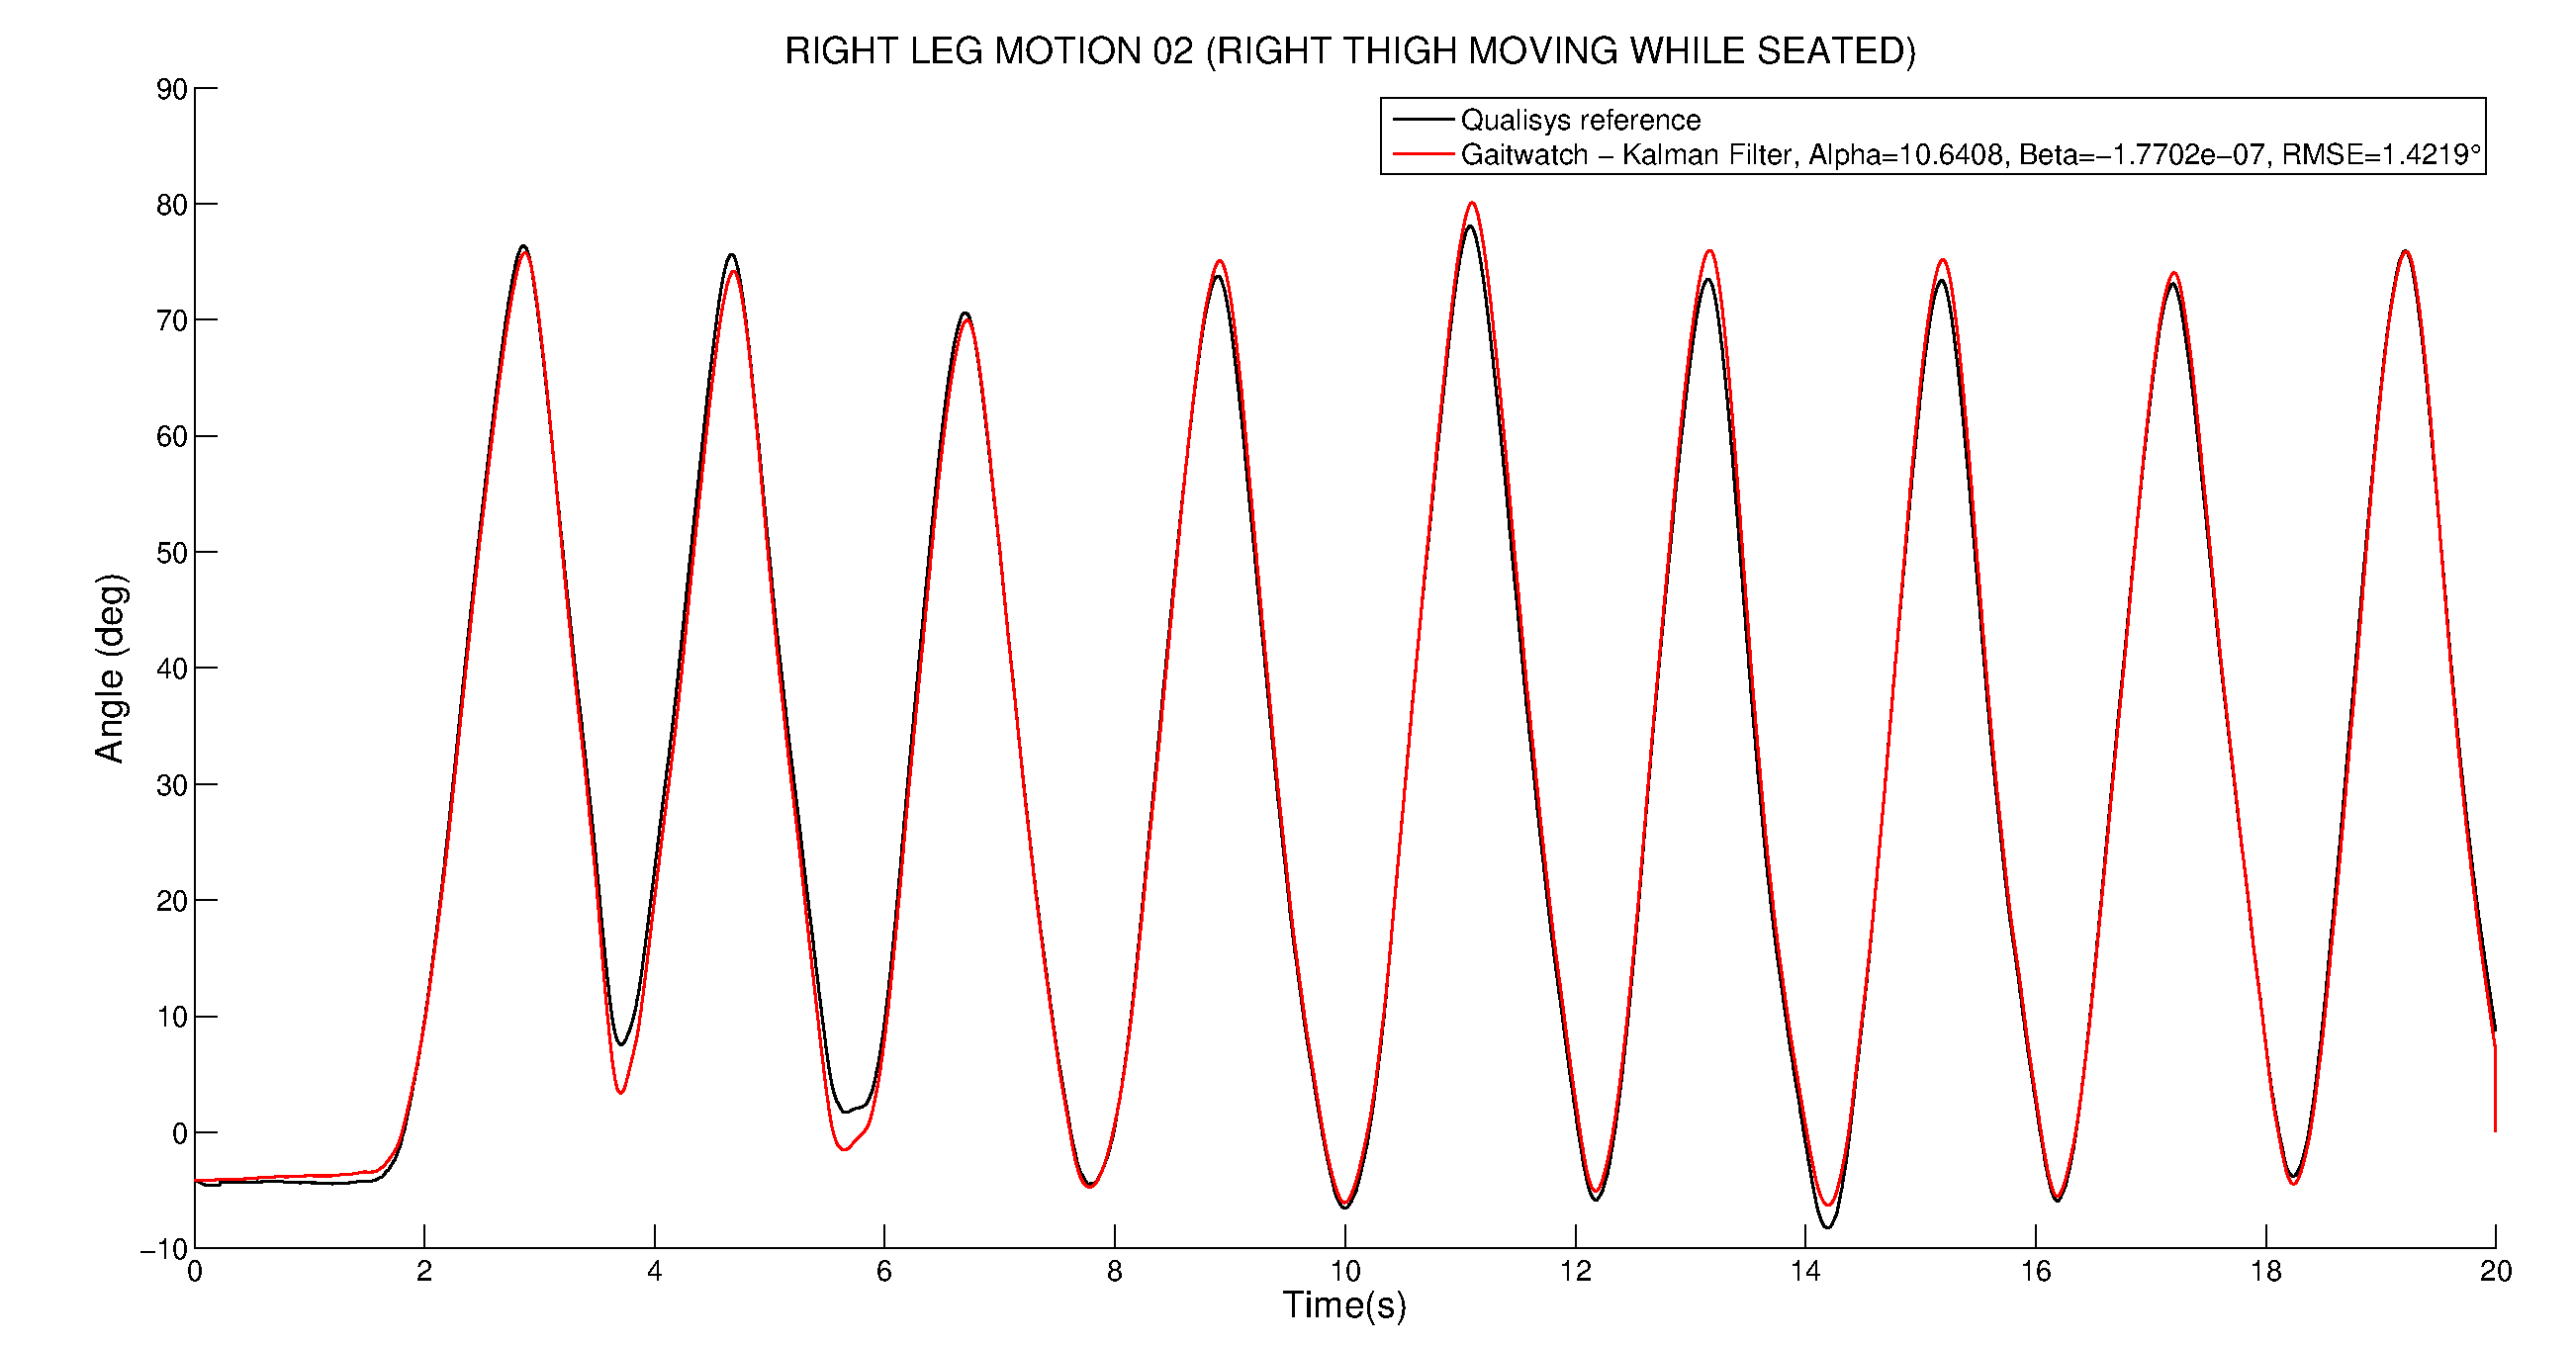
\includegraphics[width=1\textwidth]{figures/Right_leg_motion_02_thigh.eps}
\caption{Pitch angle while swinging right thigh. (GaitWatch vs. Qualisys).}
\label{fig:Right_leg_motion_02_thigh}
\end{figure}

\section{Freezing gait}

\begin{figure}[H]
\centering
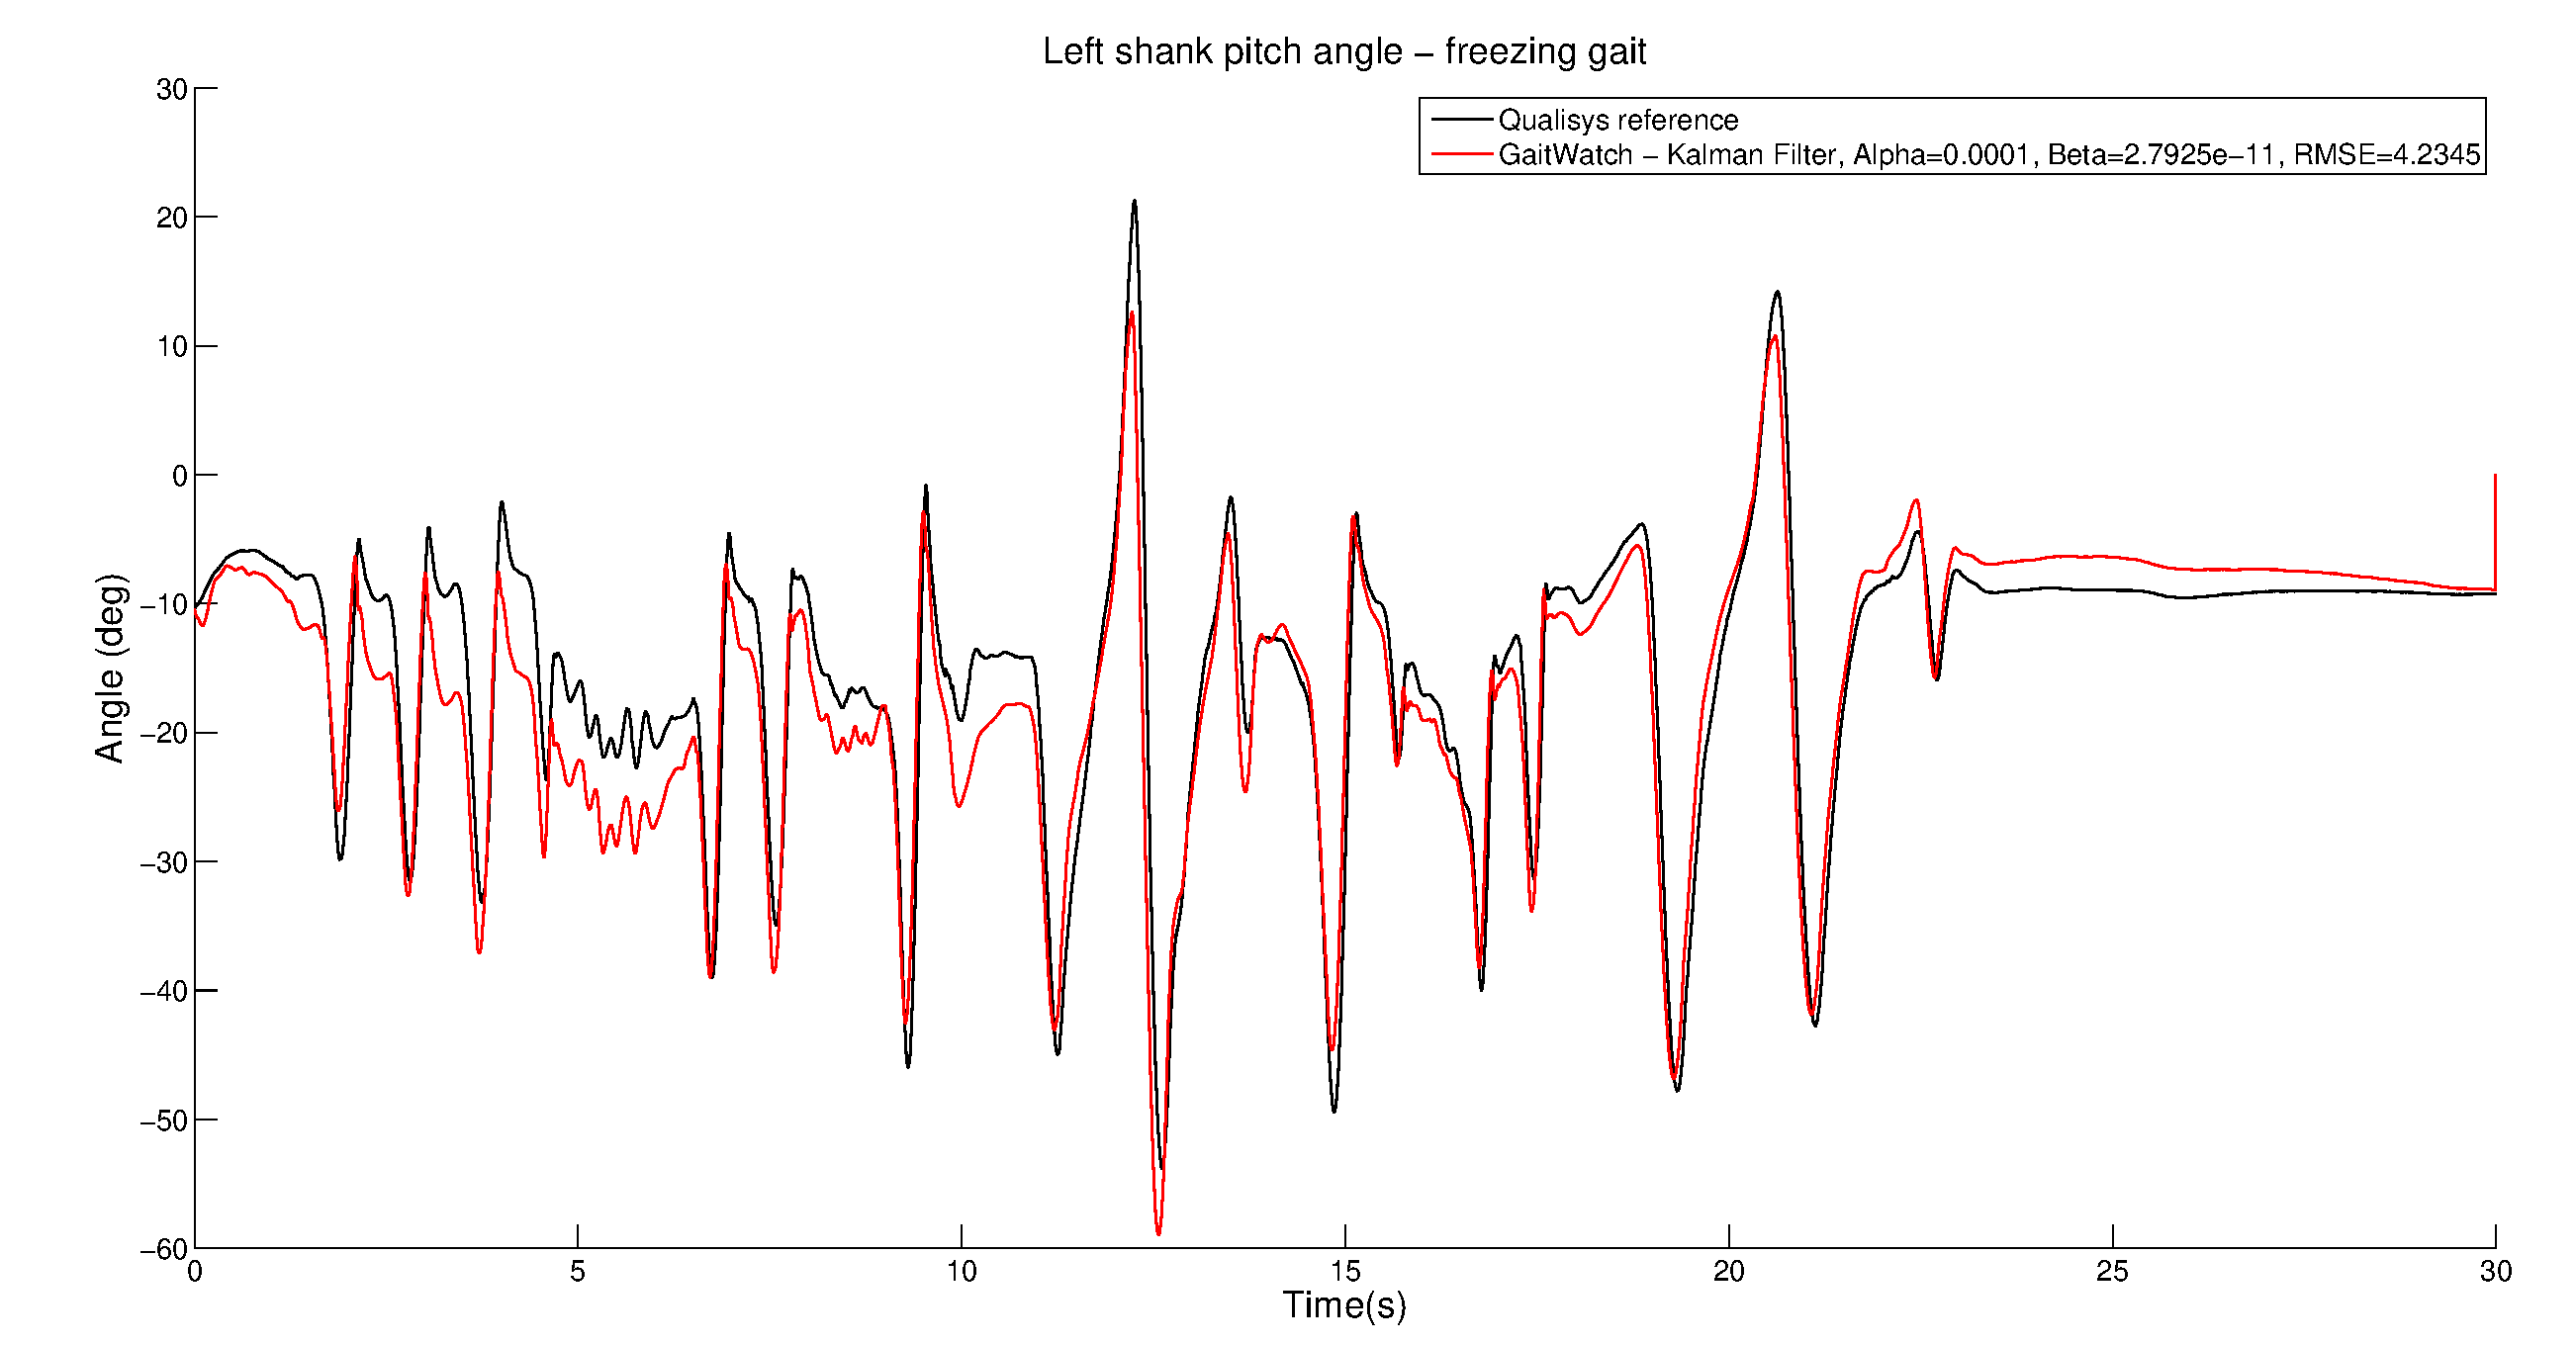
\includegraphics[width=1\textwidth]{figures/freezing_gait_left_shank.eps}
\caption{Left shank's pitch angle during freezing gait. (GaitWatch vs. Qualisys).}
\label{fig:freezing_gait_left_shank}
\end{figure}

\begin{figure}[H]
\centering
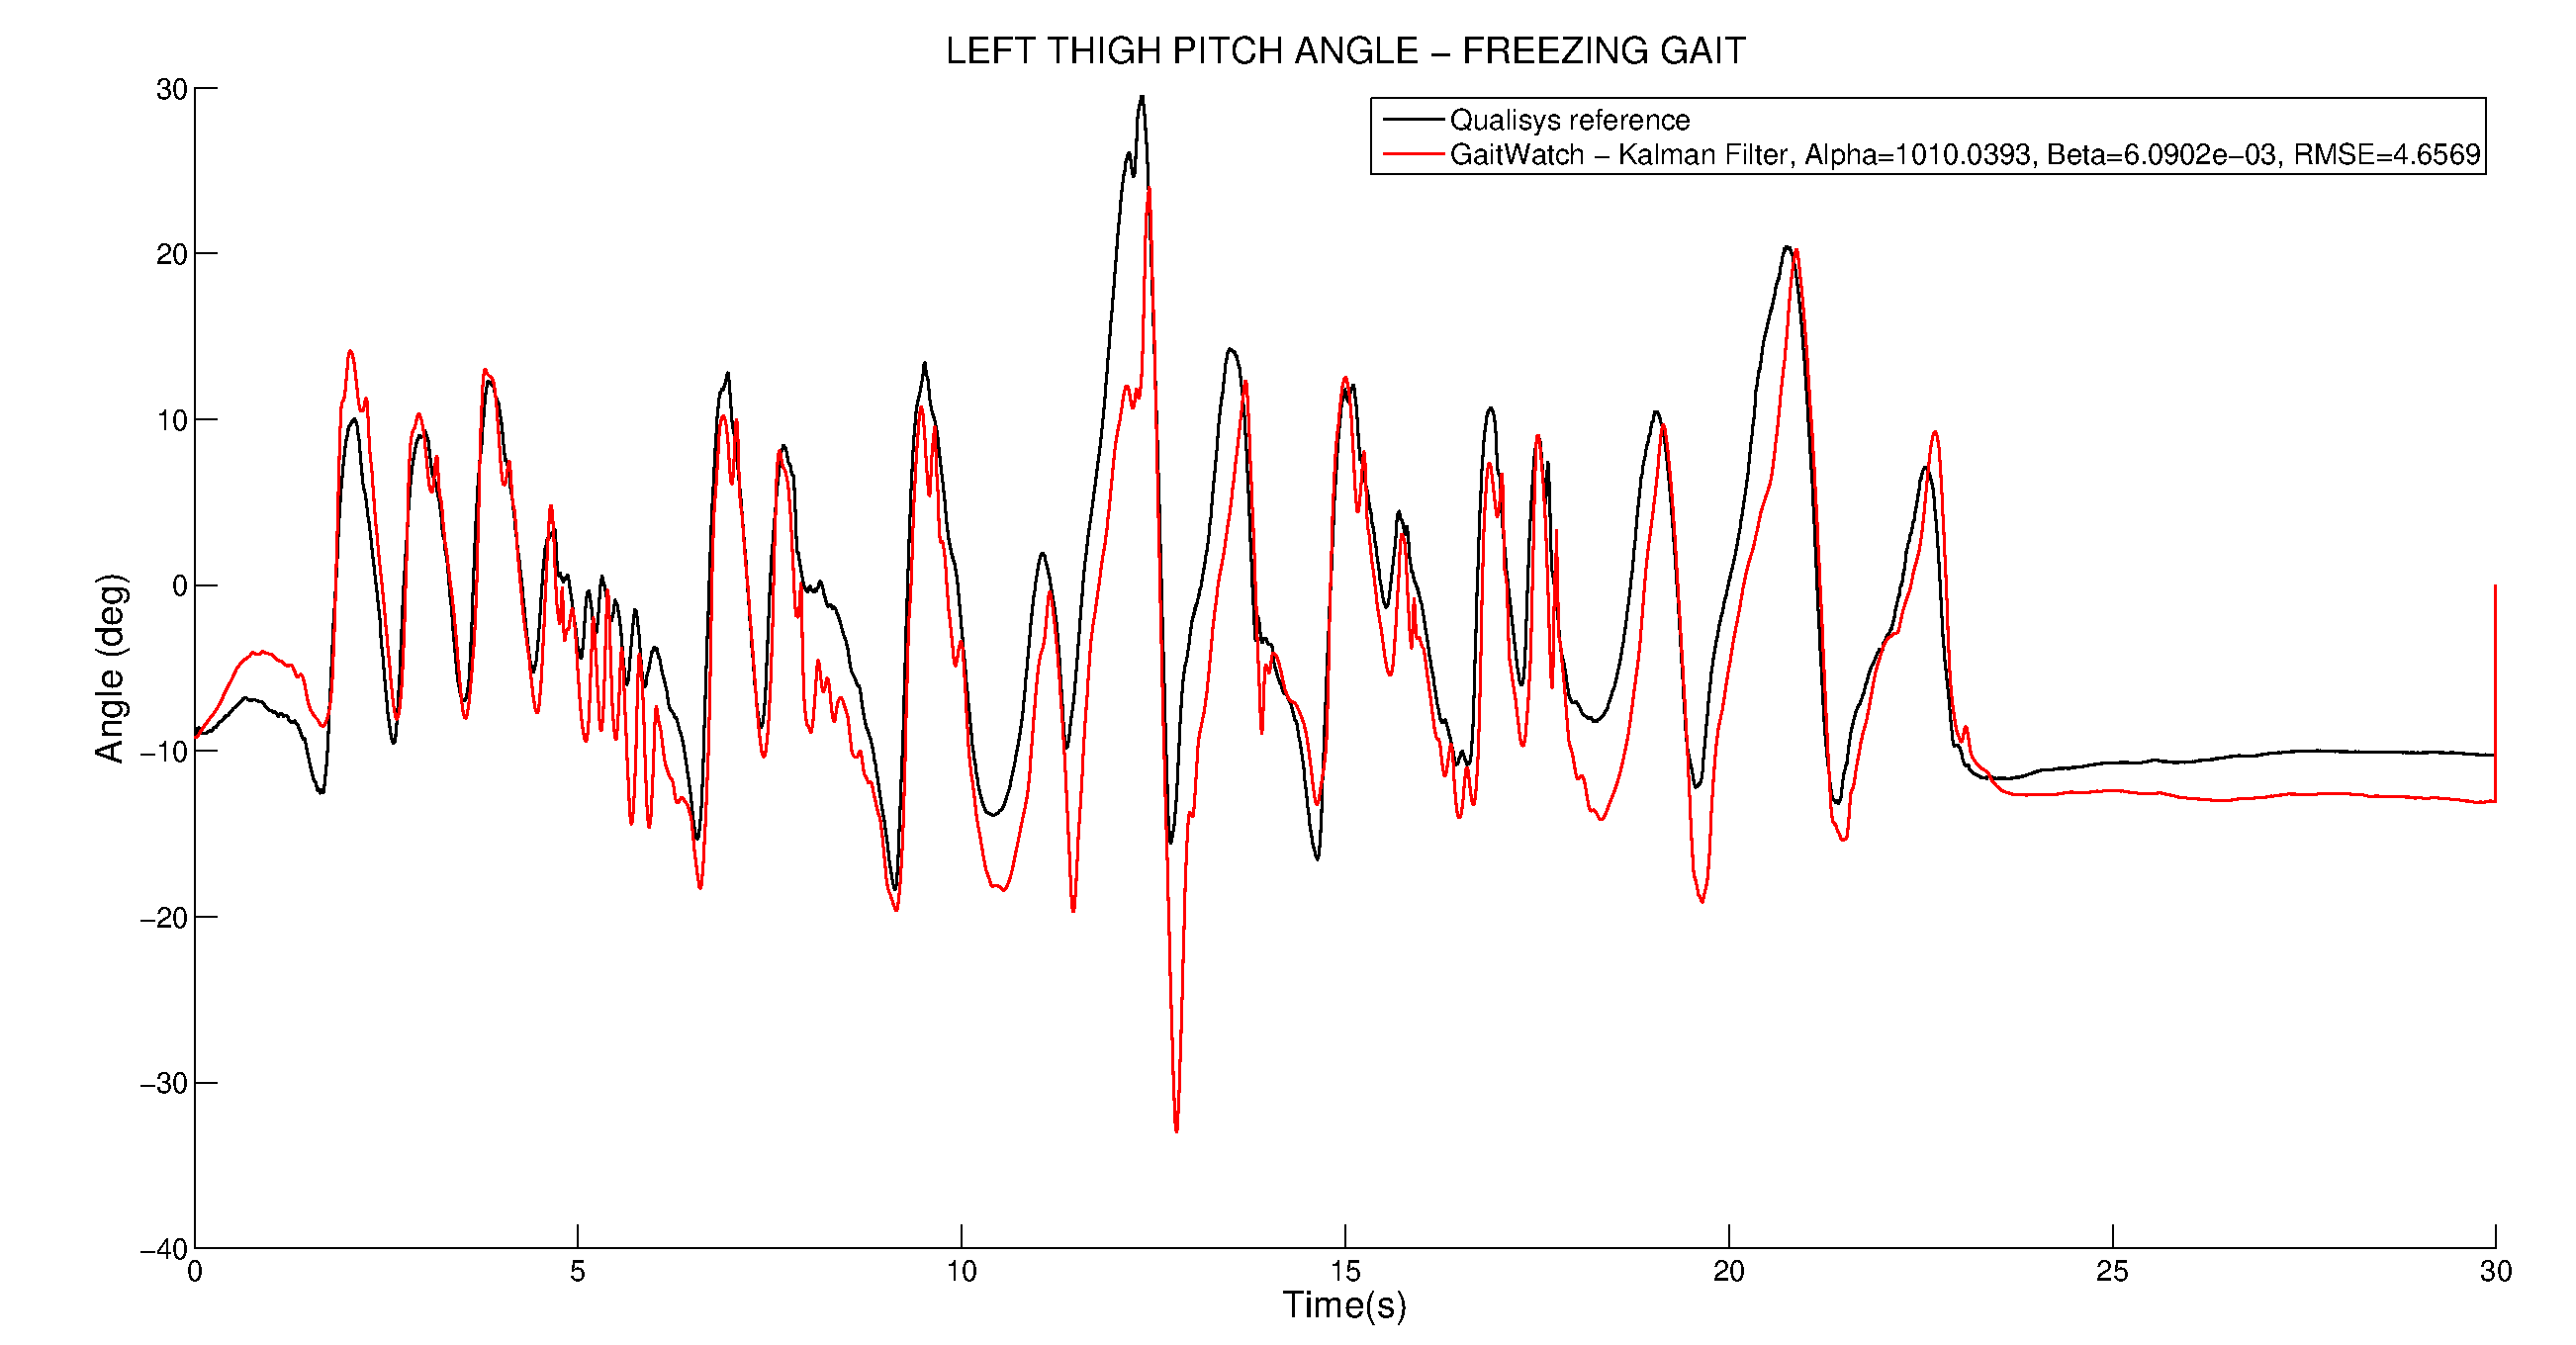
\includegraphics[width=1\textwidth]{figures/freezing_gait_left_thigh.eps}
\caption{Left thigh's pitch angle during freezing gait. (GaitWatch vs. Qualisys).}
\label{fig:freezing_gait_left_thigh}
\end{figure}

\begin{figure}[H]
\centering
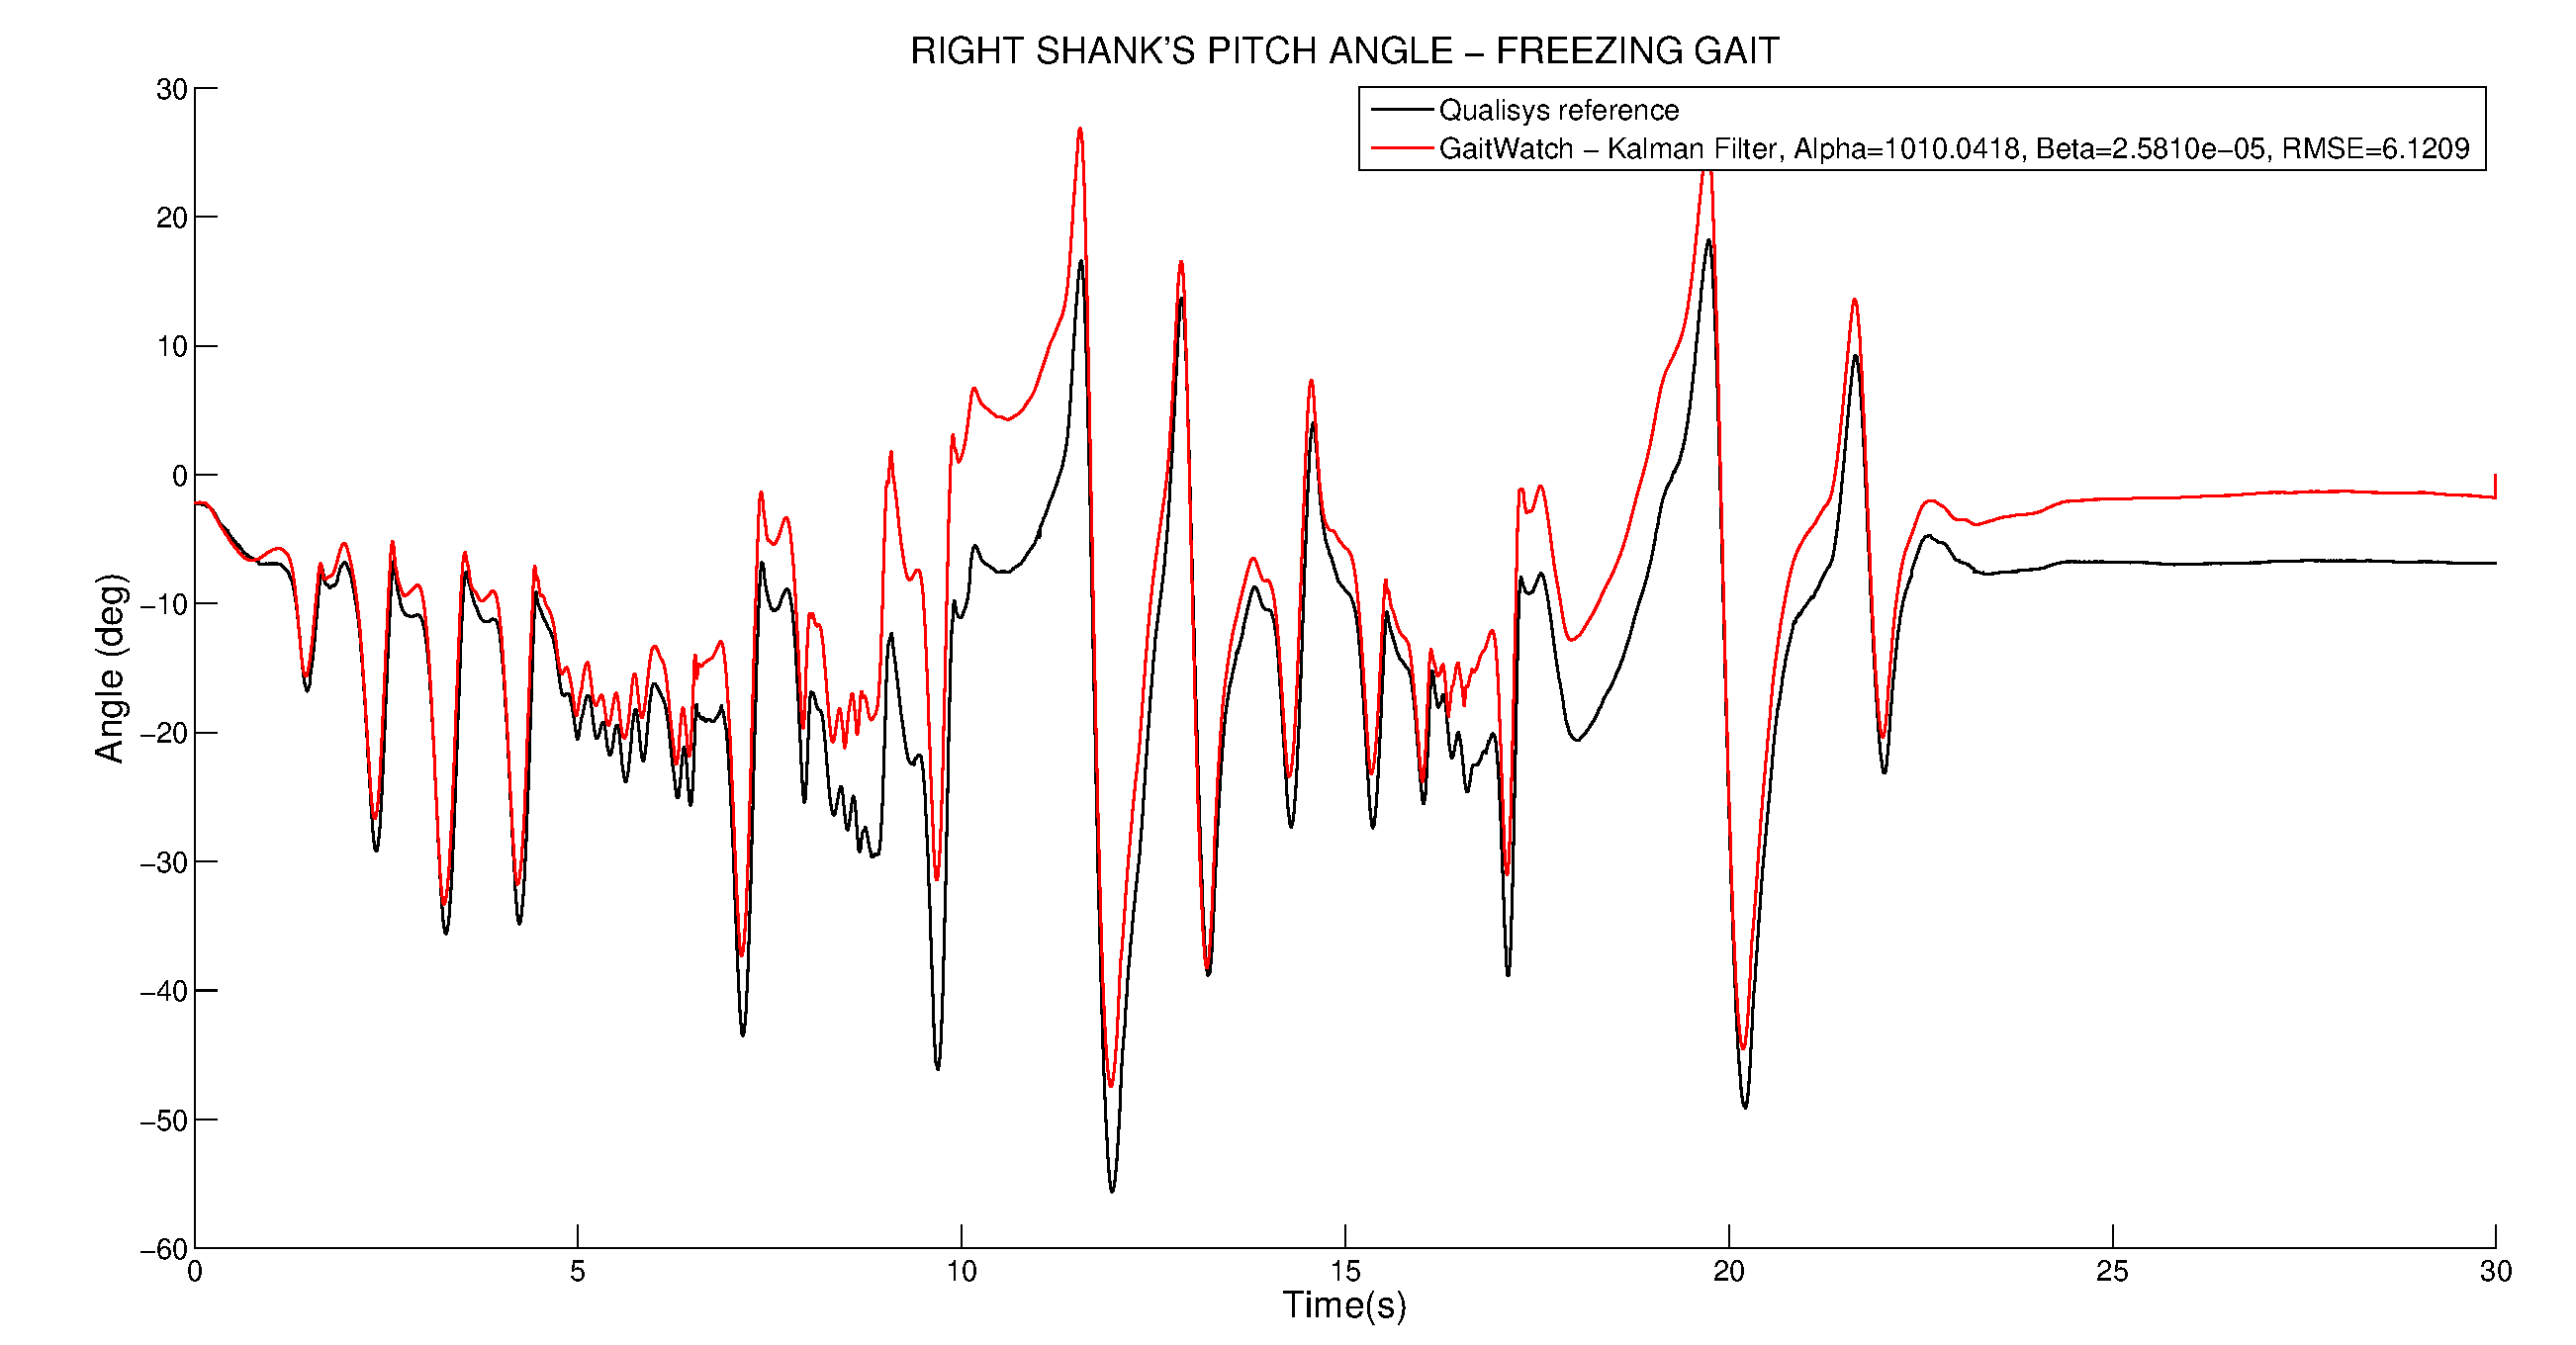
\includegraphics[width=1\textwidth]{figures/freezing_gait_right_shank.eps}
\caption{Right shank's pitch angle during freezing gait. (GaitWatch vs. Qualisys).}
\label{fig:freezing_gait_right_shank}
\end{figure}

\begin{figure}[H]
\centering
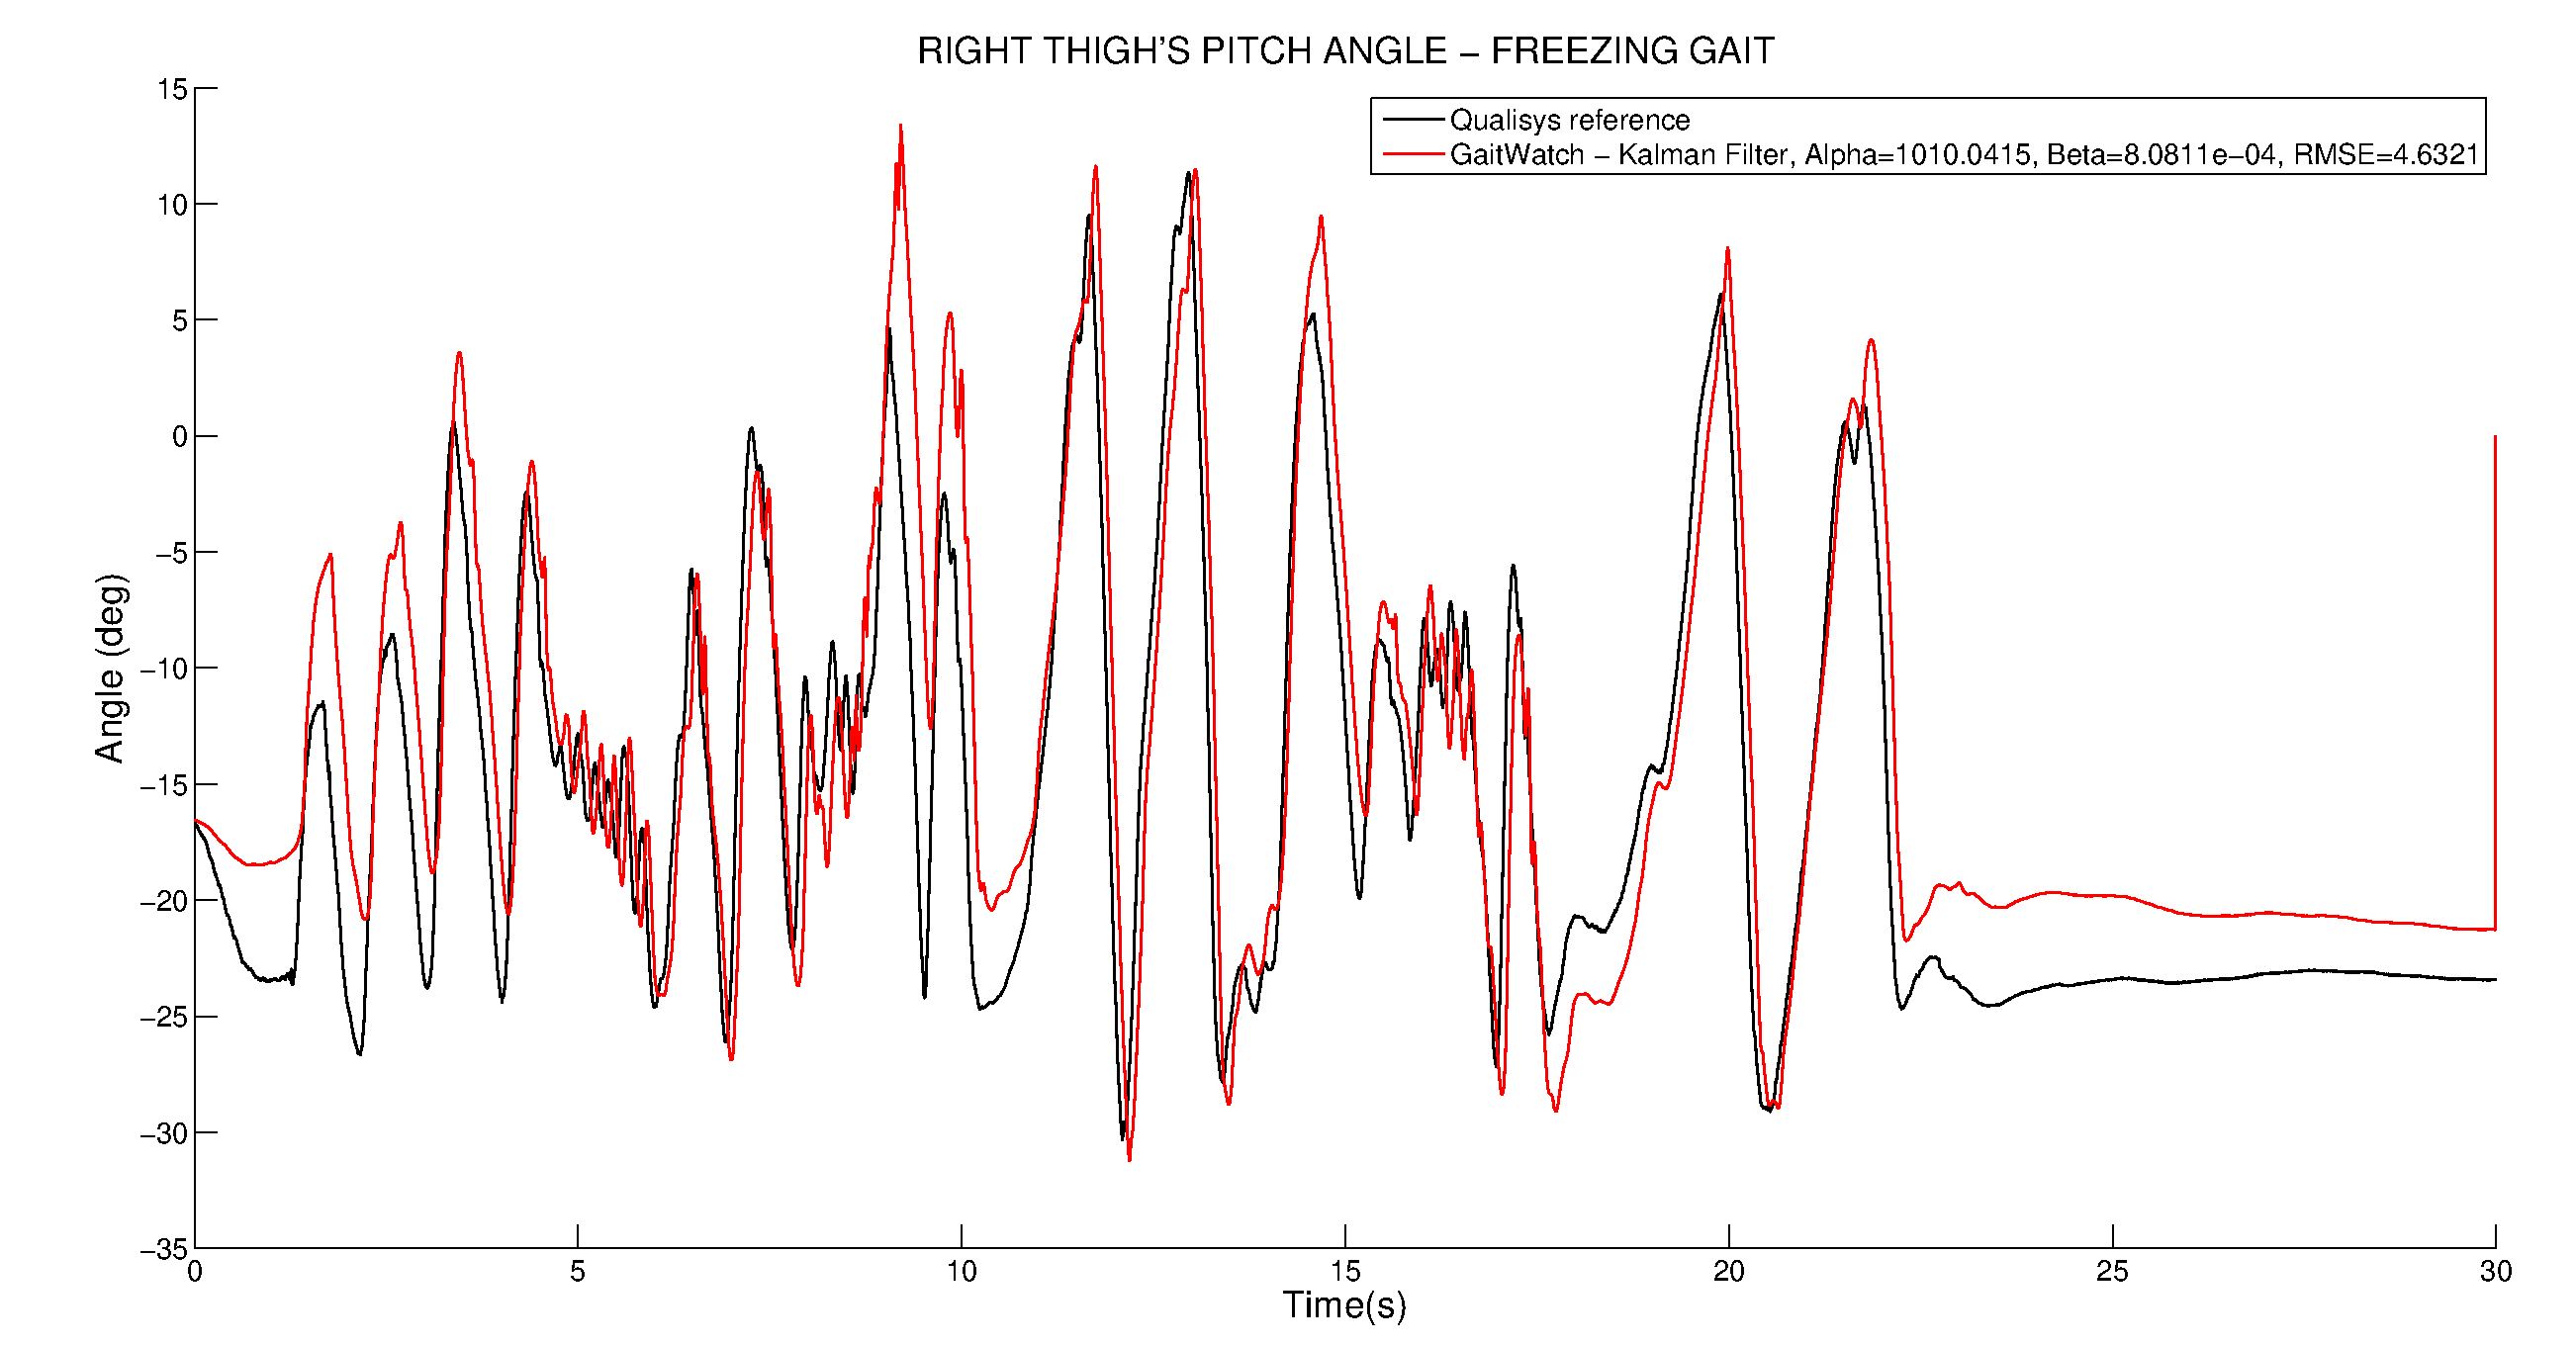
\includegraphics[width=1\textwidth]{figures/freezing_gait_right_thigh.eps}
\caption{Right thigh's pitch angle during freezing gait. (GaitWatch vs. Qualisys).}
\label{fig:freezing_gait_right_thigh}
\end{figure}

\section{Normal gait}

\begin{figure}[H]
\centering
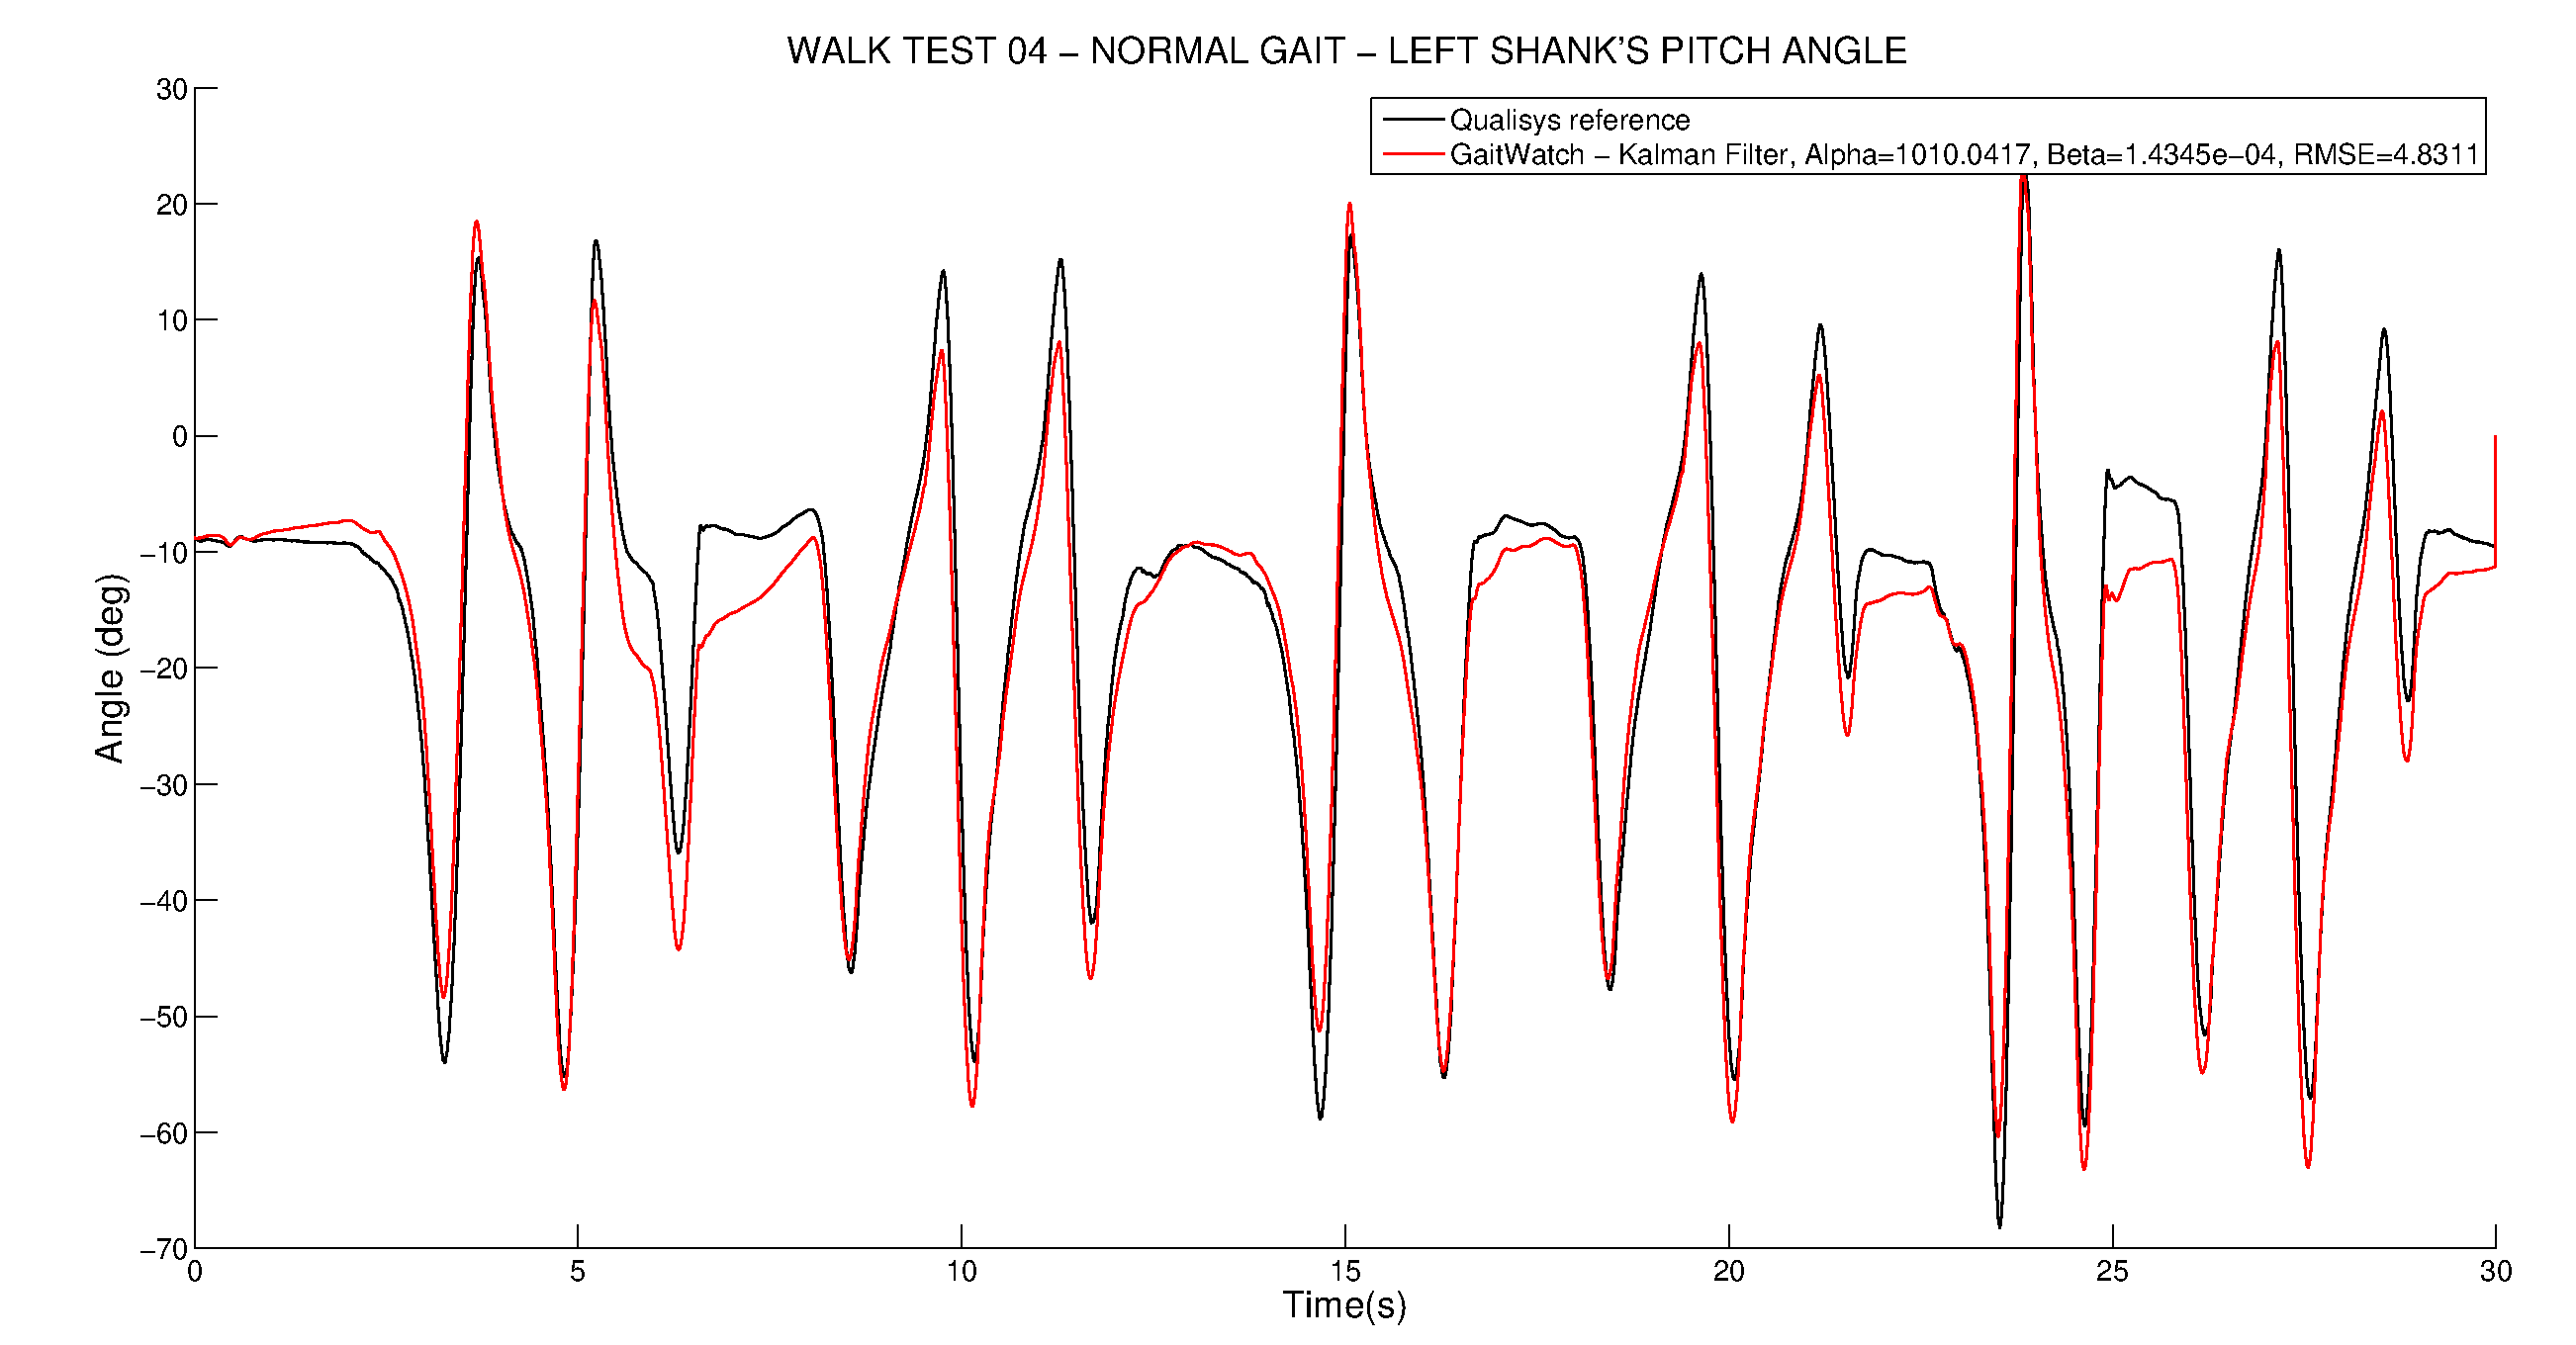
\includegraphics[width=1\textwidth]{figures/Walking_04_left_shank.eps}
\caption{Left shank's pitch angle during normal gait. (GaitWatch vs. Qualisys).}
\label{fig:Walking_04_left_shank}
\end{figure}

\begin{figure}[H]
\centering
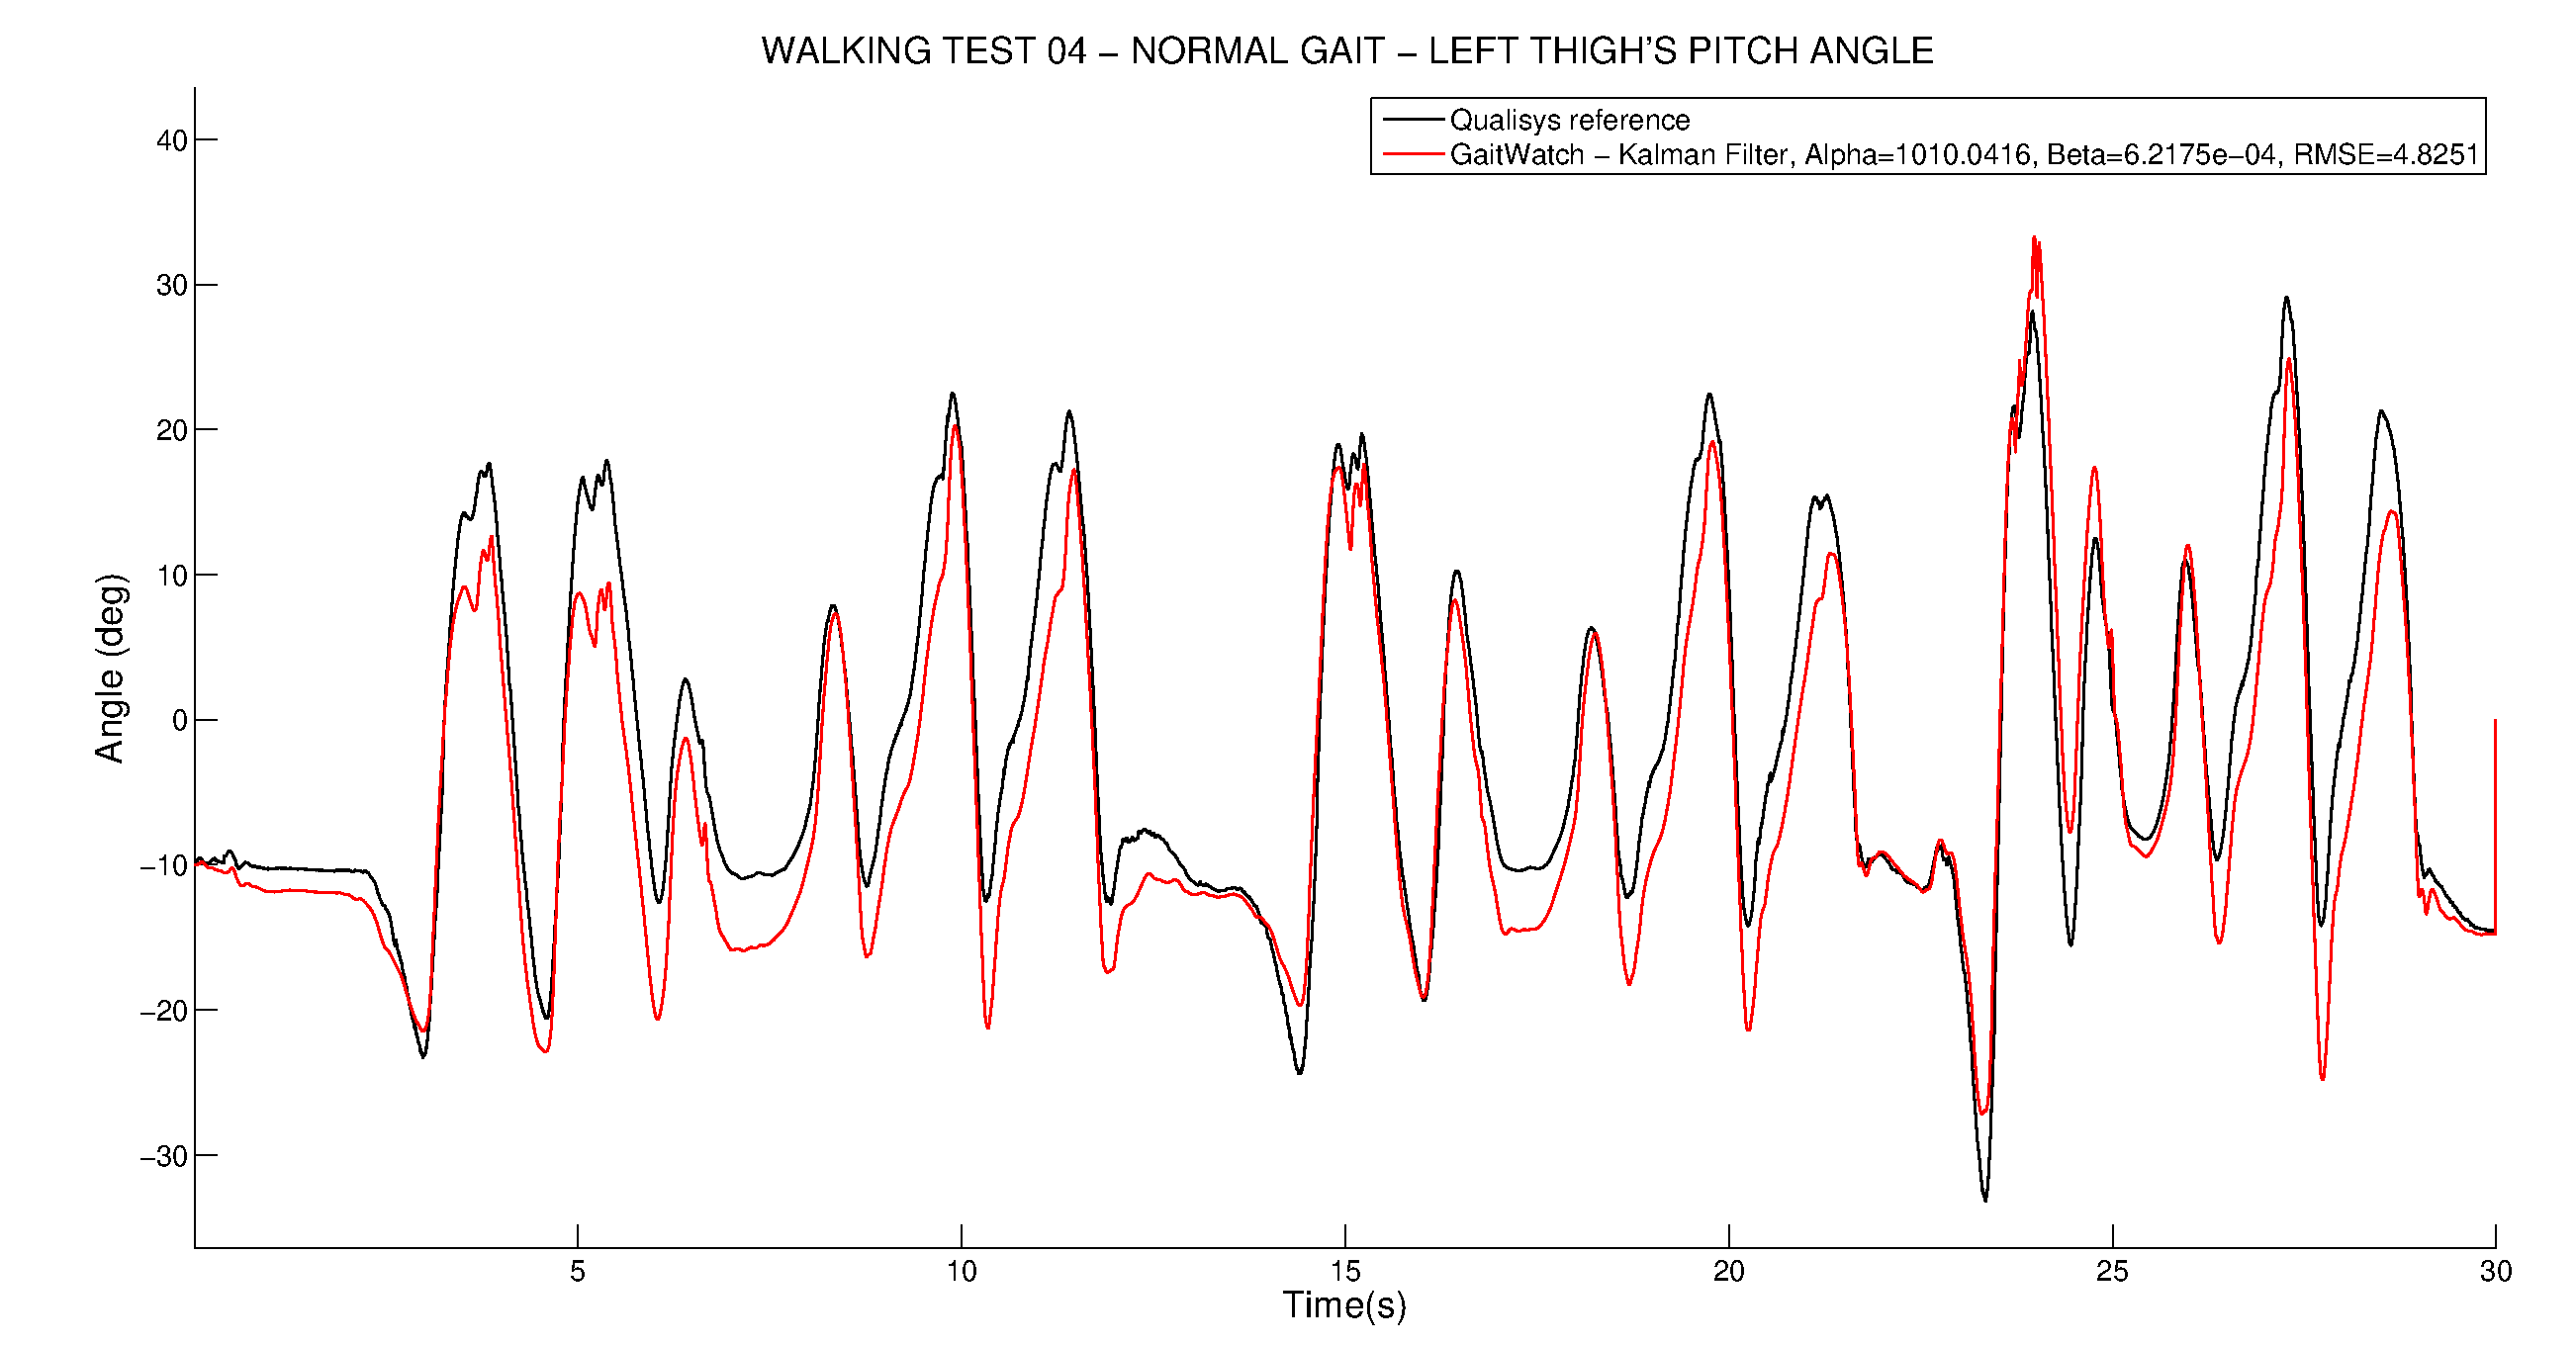
\includegraphics[width=1\textwidth]{figures/Walking_04_left_thigh.eps}
\caption{Left thigh's pitch angle during normal gait. (GaitWatch vs. Qualisys).}
\label{fig:Walking_04_left_thigh}
\end{figure}

\begin{figure}[H]
\centering
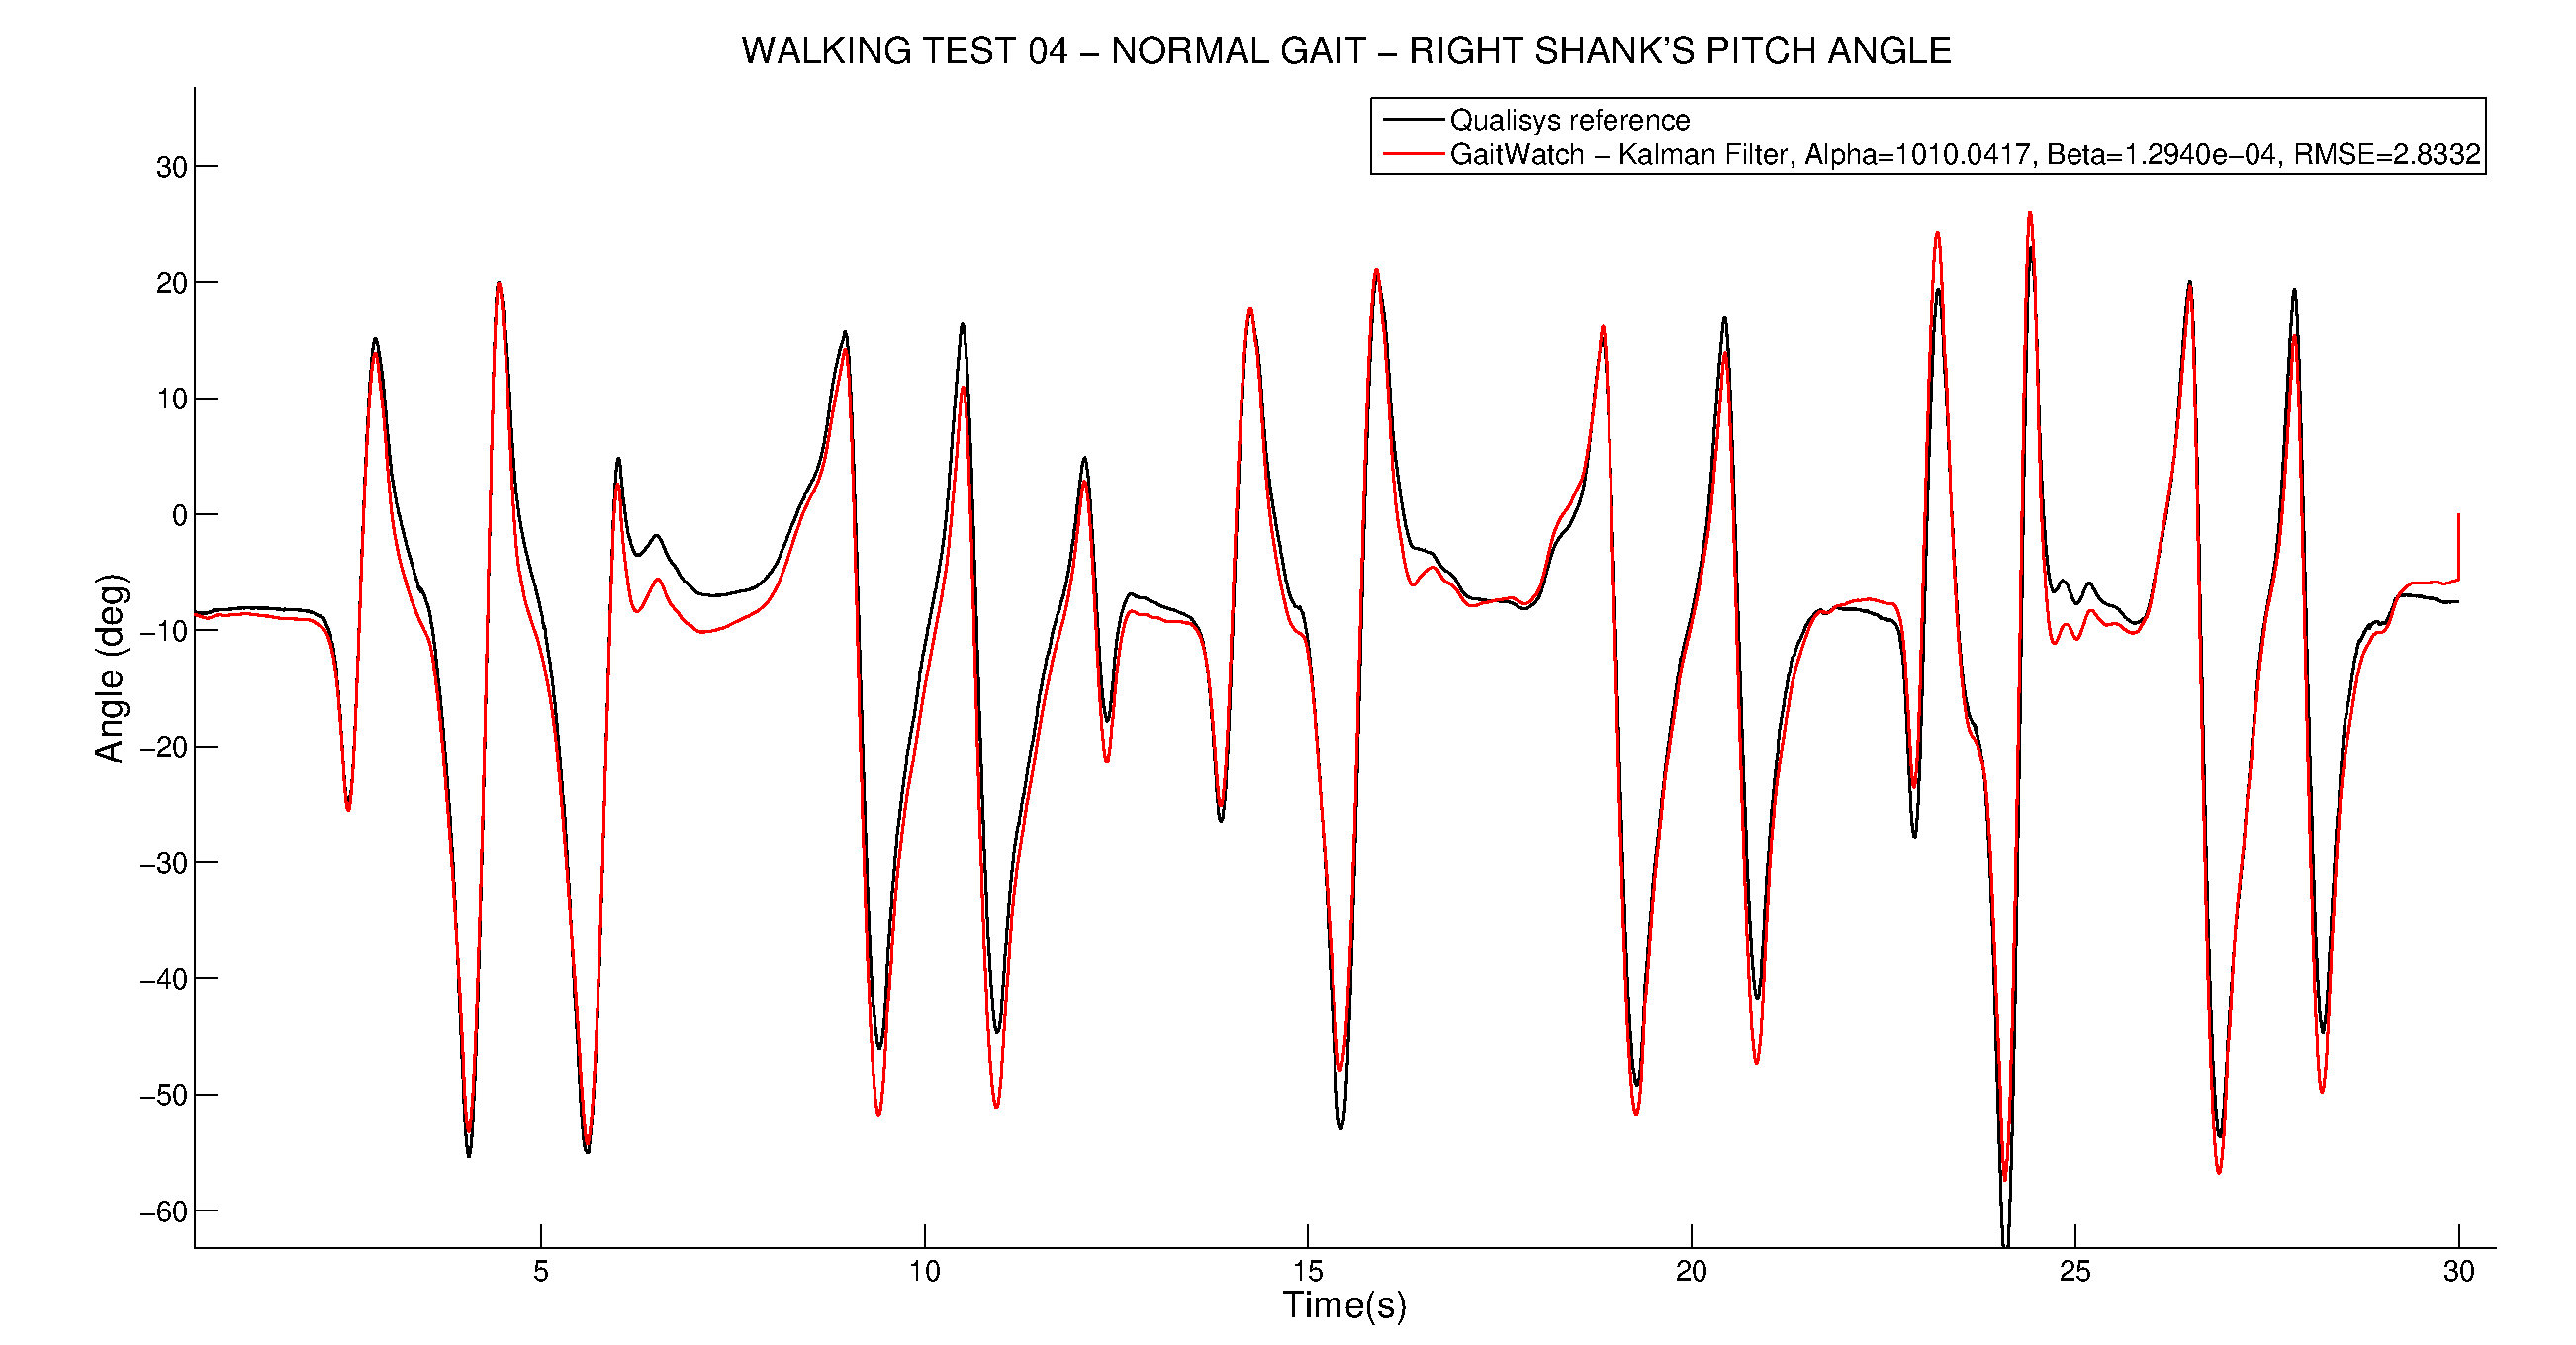
\includegraphics[width=1\textwidth]{figures/Walking_04_right_shank.eps}
\caption{Right shank's pitch angle during normal gait. (GaitWatch vs. Qualisys).}
\label{fig:Walking_04_right_shank}
\end{figure}

\begin{figure}[H]
\centering
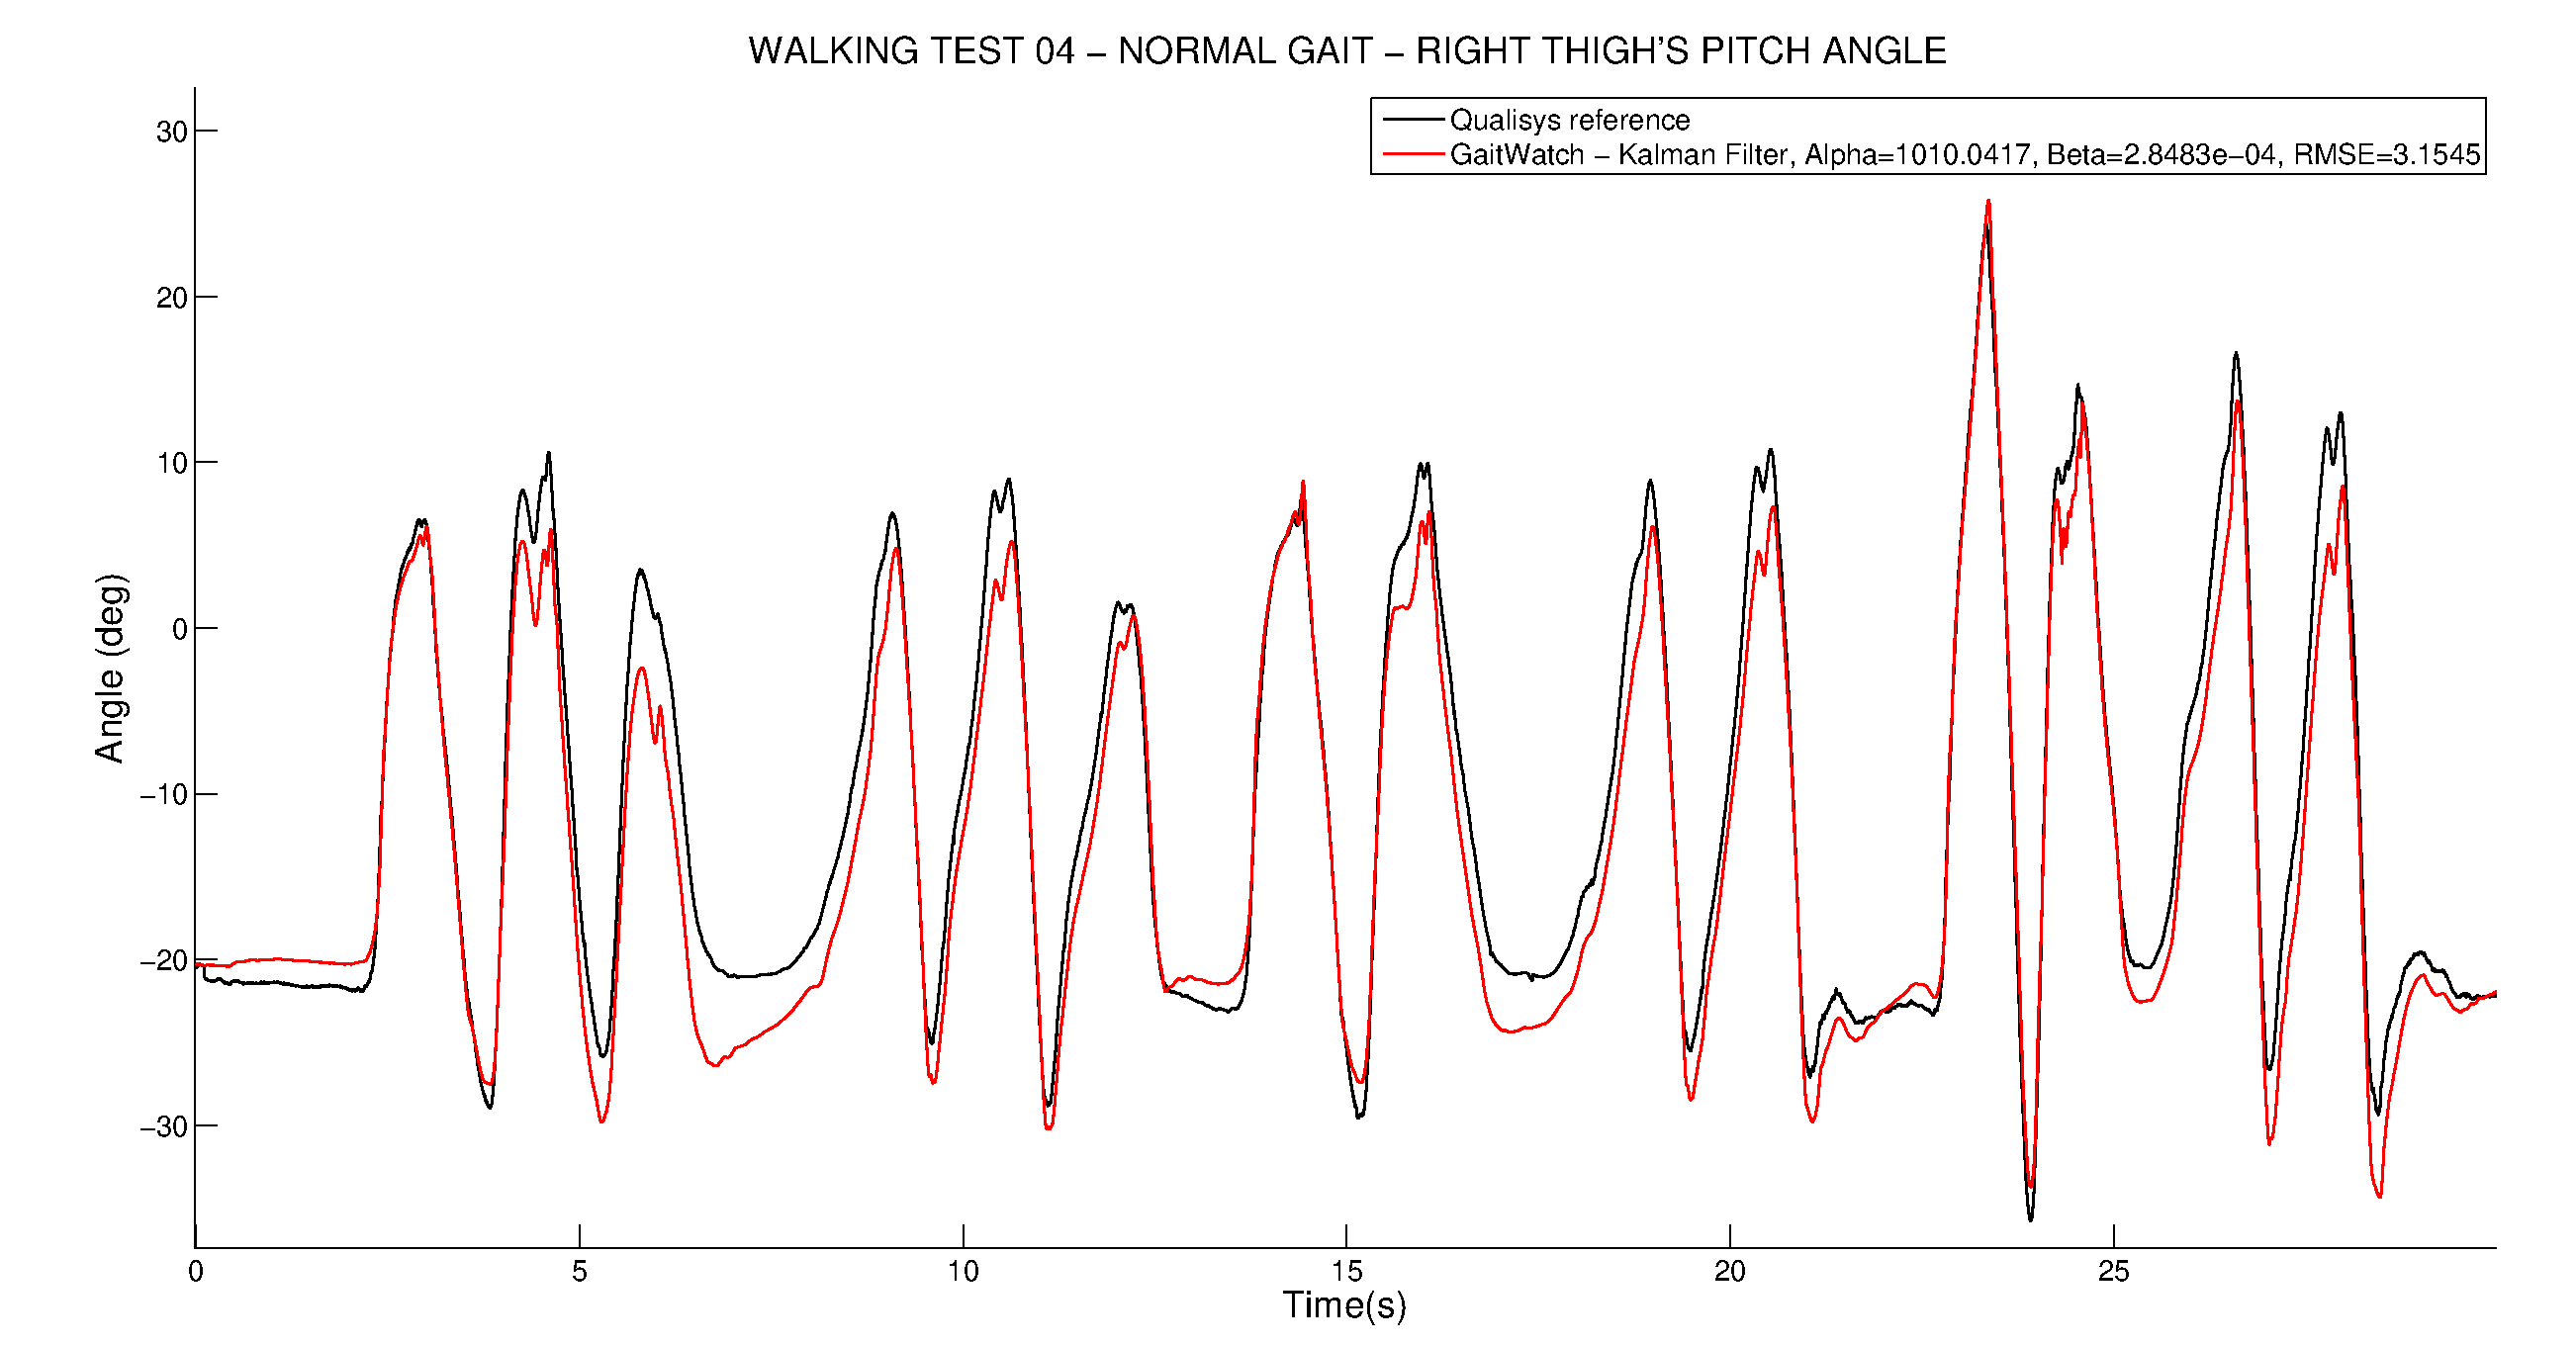
\includegraphics[width=1\textwidth]{figures/Walking_04_right_thigh.eps}
\caption{Right thigh's pitch angle during normal gait. (GaitWatch vs. Qualisys).}
\label{fig:Walking_04_right_thigh}
\end{figure}

